\documentclass[10pt,twocolumn]{article}
\usepackage[margin=0.75in]{geometry}
\usepackage{amsmath,amssymb,amsthm,booktabs,url,hyperref,graphicx,xcolor}
\newtheorem{definition}{Definition}
\newtheorem{theorem}{Theorem}
\usepackage{algorithm,algpseudocode}
\usepackage{listings}
\usepackage{enumitem}
\usepackage{balance}
\usepackage{fancyhdr}
\usepackage{titlesec}
\usepackage{pgfplots}
\pgfplotsset{compat=1.18}
\usepackage{multirow}

\titlespacing*{\section}{0pt}{1.5ex plus 0.4ex minus 0.2ex}{0.8ex plus 0.2ex}
\titlespacing*{\subsection}{0pt}{1.0ex plus 0.3ex minus 0.1ex}{0.5ex plus 0.1ex}

\setlength{\parskip}{0.4ex plus 0.15ex minus 0.1ex}
\setlength{\columnsep}{0.25in}

\lstset{
  basicstyle=\ttfamily\scriptsize,
  breaklines=true,
  frame=single,
  numbers=left,
  numberstyle=\tiny,
  captionpos=b,
  xleftmargin=1.5em,
  framexleftmargin=1.5em,
}

\hypersetup{
  colorlinks=true,
  linkcolor=blue!60!black,
  citecolor=blue!60!black,
  urlcolor=blue!60!black,
}

\newcommand{\safestep}{\textsc{SafeStep}}
\newcommand{\ie}{\textit{i.e.}}
\newcommand{\eg}{\textit{e.g.}}
\newcommand{\cf}{\textit{cf.}}

\title{\textbf{SafeStep: Verified Deployment Plans with Rollback Safety Envelopes via Bounded Model Checking}}

\author{Anonymous Authors \\ (Double-Blind Review)}
\date{}

\begin{document}

\maketitle

% ============================================================
% ABSTRACT
% ============================================================
\begin{abstract}
Deploying updates across multi-service systems is error-prone:
a single incompatible version pairing can cascade into a
cluster-wide outage, and operators often lack formal guarantees
that rollback is even possible from intermediate deployment states.
We present \safestep{}, a tool that pre-computes
\emph{rollback safety envelopes}---maximal sets of intermediate
configurations from which the system can safely revert to its
last-known-good state---for multi-service Kubernetes deployments.
\safestep{} models the deployment state space as a
\emph{version-product graph}, encodes compatibility constraints
from schema analysis, and applies SAT-based bounded model
checking (BMC) with an interval-compressed clause encoding that
achieves $O(\log^{2} L)$ clauses per service pair versus the
$O(L^{2})$ na\"ive encoding.
A \emph{monotone sufficiency theorem} guarantees that restricting
search to monotone plans is complete under downward-closed
compatibility, reducing the planning horizon.
In synthetic benchmarks calibrated against production topologies,
\safestep{} scales to 50-service clusters (0.11\,s), achieves
a 95\% success rate across 20 realistic deployment scenarios
(versus 90\% for topological-sort planning and 85\% for greedy
resource scheduling), and reduces average deployment time by
54\% through parallel execution planning (29.9\,min versus
64.9\,min for sequential baselines); note that this time
reduction is primarily attributable to \safestep{}'s ability to
batch independent services into parallel groups, rather than to
constraint-solving novelty per se.
All evaluations, including the chaos engineering validation, use
simulation models rather than live Kubernetes clusters.
\safestep{} is open-source and integrates with Helm, ArgoCD,
and Flux.
\end{abstract}

% ============================================================
% 1. INTRODUCTION
% ============================================================
\section{Introduction}
\label{sec:intro}

Modern cloud-native applications are composed of tens to
hundreds of microservices, each evolving on independent release
cadences. Deploying a coordinated update across such a system
requires traversing a combinatorial state space of service
versions, where any intermediate configuration must maintain
inter-service compatibility. When something goes wrong, operators
need to roll back---but rollback itself can fail if the system
has entered a configuration from which no safe reverse path
exists.

\paragraph{Motivating Incidents.}
The severity of deployment-induced outages is well documented.
In February~2017, an engineer at Amazon Web Services
inadvertently removed a larger set of S3 billing servers than
intended during a routine debugging exercise, triggering a
cascading failure that disrupted services across the US-East-1
region for nearly five hours~\cite{aws-s3-2017}. The root cause
was a human error in a manual deployment procedure that lacked
automated safety checks.

In June~2022, Google Cloud experienced a prolonged outage of
its Cloud SQL service when a multi-step configuration rollback
entered a stuck state: the system reached an intermediate
configuration from which neither forward progress nor safe
reversion was possible~\cite{gcloud-sql-2022}. The incident
required manual intervention spanning multiple hours and affected
hundreds of customer databases.

Cloudflare's July~2019 outage was triggered by deploying a
regular expression rule that caused catastrophic CPU exhaustion
across its global edge network~\cite{cloudflare-2019}. The
faulty rule passed staging tests but interacted pathologically
with production traffic patterns. A rapid rollback was possible
only because the deployment topology happened to support it---no
formal analysis had verified this property.

In November~2020, AWS Kinesis experienced a multi-hour outage
when a capacity scaling operation exceeded the maximum number
of threads permitted by the operating system, creating a
cascading failure across front-end servers~\cite{aws-kinesis-2020}.
The deployment plan had no formal model of the interaction
between capacity parameters and OS-level constraints.

\paragraph{The Gap.}
These incidents share a common thread: the absence of formal
reasoning about deployment safety. Existing tools---Helm~\cite{helm},
ArgoCD~\cite{argocd}, Flux~\cite{flux}, and Terraform~\cite{terraform}---automate
the \emph{execution} of deployment plans but do not \emph{verify}
that every intermediate state is safe or that rollback is possible.
Canary deployments and progressive delivery frameworks such as
Argo Rollouts~\cite{argo-rollouts} and Flagger~\cite{flagger}
mitigate risk by limiting blast radius, but they cannot guarantee
the absence of stuck configurations. The deployment planning
problem is fundamentally combinatorial, and ad hoc operational
procedures are insufficient.

\paragraph{Microservice deployment challenges.}
The challenges of microservice deployment have been widely
recognized~\cite{taibi-microservices-2017}. Taibi et al.\ identify
coordination complexity as a primary concern: as the number of
independently deployable services grows, the number of
pairwise interactions grows quadratically, and the space of
possible version combinations grows exponentially. In a system
with $n$ services and $L$ versions each, the total
configuration space has $L^n$ states. Even modest systems
(20~services, 10~versions) have $10^{20}$ possible
configurations---far beyond what can be explored by manual
analysis or simple heuristics.

The problem is exacerbated by the velocity of modern
software delivery. Schermann et al.~\cite{schermann-progressive-2018}
report that organizations practicing continuous deployment
release updates multiple times per day, often without full
integration testing of all version combinations. The result is
that production systems routinely traverse untested
configurations during deployment, and operators rely on
observational monitoring (metrics, logs, traces) to detect
problems after they occur. This reactive approach is inherently
limited: by the time a problem is detected, the system may
already be in a stuck configuration from which recovery is
difficult.

\paragraph{The case for formal verification.}
We argue that deployment safety is a verification problem, not
a testing problem. Testing can increase confidence that a
deployment will succeed, but it cannot prove the absence of
failure---especially for multi-step deployments where the number
of intermediate configurations is combinatorial. Formal
verification, by contrast, can provide mathematical guarantees
that every intermediate state satisfies safety properties.
Bounded model checking (BMC)~\cite{biere-bmc-2003} is
particularly well-suited to this domain: deployment plans
have bounded length (at most $\sum_i L_i$ steps), the state
space is finite (though exponentially large), and the safety
properties are naturally expressible as propositional
constraints.

\paragraph{Scope and applicability.}
\safestep{} targets \emph{planned, coordinated deployments}
where multiple services are updated in a single maintenance
window. This is the deployment model used by most organizations
for major version upgrades, database schema migrations, and
breaking API changes. For independent single-service deployments
(where each service can be updated without affecting others),
\safestep{}'s analysis is trivially satisfied and the tool
adds no value beyond confirming the absence of cross-service
constraints. The tool is most valuable in the ``middle ground''
that characterizes real-world systems: partially coupled services
with complex version compatibility requirements that are
difficult for humans to reason about manually.

\paragraph{Our Approach.}
We introduce \safestep{}, a tool that fills this gap by
applying bounded model checking (BMC)~\cite{biere-bmc-2003} to
deployment planning. \safestep{} models the deployment state
space as a \emph{version-product graph} $G = (V, E)$, where
each vertex represents a global configuration (a tuple of
per-service versions) and edges represent single-service
upgrade or downgrade steps. Inter-service compatibility
constraints, derived from schema analysis, define the \emph{safe
subgraph}. A deployment plan is a path in this subgraph from
the current configuration to the target, and a \emph{rollback
safety envelope} is the maximal set of vertices along the plan
from which the start configuration is reachable within the safe
subgraph.

\safestep{} uses a novel \emph{interval-compressed encoding}
that represents version-ordering constraints in $O(\log^{2} L)$
clauses per service pair (where $L$ is the maximum number of
versions per service), compared to $O(L^{2})$ for the na\"ive
encoding. A \emph{monotone sufficiency theorem} proves that
restricting search to monotone (non-decreasing) plans is complete
under the common assumption of downward-closed compatibility,
reducing the BMC horizon to $k^{*} = \sum_{i}(g_{i} - s_{i})$,
where $g_{i}$ and $s_{i}$ are the goal and start version indices
for service $i$.

\paragraph{Contributions.}
This paper makes the following contributions:
\begin{enumerate}[leftmargin=*,nosep]
  \item The concept of \emph{rollback safety envelopes} for
        multi-service deployments (Section~\ref{sec:problem}).
  \item An \emph{interval-compressed BMC encoding} with
        $O(\log^{2} L)$ clauses per service pair
        (Section~\ref{sec:approach}).
  \item A \emph{monotone sufficiency theorem} that establishes
        completeness of monotone planning under downward-closed
        compatibility, with a tight BMC completeness threshold
        (Section~\ref{sec:approach}).
  \item \safestep{}, an open-source implementation in Rust
        with integrations for Helm, Kustomize, ArgoCD, and Flux
        (Section~\ref{sec:impl}).
\end{enumerate}

% ============================================================
% 2. BACKGROUND & PROBLEM DEFINITION
% ============================================================
\section{Background \& Problem Definition}
\label{sec:problem}

\subsection{Version-Product Graphs}

Consider a system of $n$ services $S = \{s_1, \ldots, s_n\}$.
Each service $s_i$ has an ordered set of versions
$\mathcal{V}_i = \{v_i^0, v_i^1, \ldots, v_i^{L_i}\}$,
where $v_i^0$ is the currently deployed version and $v_i^{L_i}$
is the target version. The \emph{version-product graph} is:

\begin{definition}[Version-Product Graph]
$G = (V, E)$ where the vertex set $V = \mathcal{V}_1 \times
\mathcal{V}_2 \times \cdots \times \mathcal{V}_n$ is the
Cartesian product of per-service version sets, and the edge
set $E$ connects configurations that differ in exactly one
service by one version step:
\[
  E = \{(u, u') \mid \exists!\, i : u'_i = u_i \pm 1,\;
        \forall j \neq i : u'_j = u_j\}
\]
\end{definition}

The total number of vertices is $|V| = \prod_{i=1}^{n} (L_i + 1)$,
which is exponential in $n$. Explicit enumeration is infeasible
for realistic systems; symbolic methods are essential.

\subsection{Compatibility and Safe States}

Inter-service compatibility is specified by a \emph{compatibility
oracle} $\mathcal{O} : V \to \{\mathsf{safe}, \mathsf{unsafe}\}$.
In practice, the oracle is constructed from API schema analysis
(protobuf, OpenAPI, GraphQL), database migration ordering, and
operator-specified constraints. A configuration $u \in V$ is
\emph{safe} if $\mathcal{O}(u) = \mathsf{safe}$.

We define $V_{\mathsf{safe}} = \{u \in V \mid \mathcal{O}(u) =
\mathsf{safe}\}$ and the \emph{safe subgraph} $G_{\mathsf{safe}}
= (V_{\mathsf{safe}}, E \cap (V_{\mathsf{safe}} \times V_{\mathsf{safe}}))$.

\begin{definition}[Downward-Closed Compatibility]
\label{def:downward}
The oracle $\mathcal{O}$ is \emph{downward-closed} if for all
$u, u' \in V$: if $u \in V_{\mathsf{safe}}$ and $u' \leq u$
componentwise, then $u' \in V_{\mathsf{safe}}$.
\end{definition}

Downward closure is a natural property: if two service versions
are compatible, then compatibility is preserved when either
service is at a lower (older, more conservative) version.
This holds for additive API evolution (new fields/endpoints)
but can be violated by breaking changes.

\subsection{Deployment Plans and Rollback Safety}

\begin{definition}[Deployment Plan]
A \emph{deployment plan} is a path $\pi = (c_0, c_1, \ldots, c_k)$
in $G_{\mathsf{safe}}$ from the start configuration $c_0 = \mathbf{s}$
to the goal configuration $c_k = \mathbf{g}$.
\end{definition}

\begin{definition}[Monotone Plan]
A plan $\pi$ is \emph{monotone} if for all consecutive states
$c_t, c_{t+1}$, the version change is non-decreasing:
$c_{t+1,i} \geq c_{t,i}$ for the unique service $i$ that changes.
\end{definition}

\begin{definition}[Rollback Safety Envelope]
\label{def:envelope}
Given a plan $\pi = (c_0, \ldots, c_k)$, the \emph{rollback
safety envelope} is
\[
  \mathcal{E}(\pi) = \{c_t \mid \exists\, \text{path from } c_t
  \text{ to } c_0 \text{ in } G_{\mathsf{safe}}\}
\]
The \emph{point of no return} is $t^{*} = \max\{t \mid c_t
\in \mathcal{E}(\pi)\}$.
\end{definition}

\noindent
\textbf{Problem Statement.}
Given a version-product graph $G$, a compatibility oracle
$\mathcal{O}$, start $\mathbf{s}$, and goal $\mathbf{g}$:
(1)~find a safe deployment plan $\pi$ from $\mathbf{s}$ to
$\mathbf{g}$ in $G_{\mathsf{safe}}$, or prove none exists;
(2)~compute the rollback safety envelope $\mathcal{E}(\pi)$ and
the point of no return $t^{*}$.

\subsection{Ordering Constraints and Resource Bounds}

In practice, deployment plans are subject to additional
constraints beyond version compatibility:

\paragraph{Service ordering constraints.}
Operators may require that certain services be upgraded before
others. For example, a database schema migration service must
be upgraded before application services that depend on the new
schema. These constraints are expressed as a partial order
$\prec$ on the set of services: $s_i \prec s_j$ means that
$s_i$ must reach its goal version before $s_j$ begins upgrading.
In the BMC encoding, ordering constraints translate to
implications: $\sigma_{j,t} \Rightarrow (x_{i,t} = g_i)$ for
all $t$ and all $(s_i, s_j)$ with $s_i \prec s_j$, where
$\sigma_{j,t}$ indicates that service $j$ steps at time $t$.

\paragraph{Resource constraints.}
During a rolling update, the cluster may temporarily run more
pods than usual (due to surge capacity). Resource constraints
limit the total memory, CPU, or pod count at any time step.
These are encoded as linear constraints
$\sum_i r_i(x_{i,t}) \leq R_{\max}$ where $r_i(v)$ is the
resource demand of service $s_i$ at version $v$. Since linear
constraints cannot be directly encoded in SAT, they are handled
by the Z3-based CEGAR refinement loop
(Section~\ref{sec:cegar}).

\paragraph{Maintenance windows.}
Some services may only be updated during designated maintenance
windows. This is modeled by restricting the time steps at which
certain services can be modified:
$\sigma_{i,t} \Rightarrow t \in W_i$, where $W_i$ is the set
of allowed time steps for service $s_i$.

% ============================================================
% 3. APPROACH
% ============================================================
\section{Approach}
\label{sec:approach}

\subsection{Architecture Overview}

\safestep{} comprises five components in a pipeline
architecture:

\begin{enumerate}[leftmargin=*,nosep]
  \item \textbf{Schema Oracle}: Parses API schemas (protobuf,
    OpenAPI, GraphQL), database migrations, and operator
    annotations to construct the compatibility oracle
    $\mathcal{O}$.
  \item \textbf{Constraint Encoder}: Translates $\mathcal{O}$
    and the version-product graph structure into a
    propositional formula using the interval-compressed
    encoding (Section~\ref{sec:encoding}).
  \item \textbf{BMC Engine}: Performs bounded model checking
    using CaDiCaL~\cite{cadical} as the SAT solver, with
    incremental unrolling up to the completeness threshold
    $k^{*}$ (Theorem~\ref{thm:completeness}).
  \item \textbf{Envelope Analyzer}: Given a plan $\pi$, computes
    the rollback safety envelope $\mathcal{E}(\pi)$ by solving
    a series of reachability queries on the safe subgraph.
  \item \textbf{Output Module}: Generates deployment manifests
    (Helm values, Kustomize overlays, ArgoCD ApplicationSets)
    annotated with rollback safety metadata.
\end{enumerate}

\subsection{Key Theorems}

\begin{theorem}[Monotone Sufficiency]
\label{thm:monotone}
If the compatibility oracle $\mathcal{O}$ is downward-closed
(Definition~\ref{def:downward}), then for every safe deployment
plan $\pi$ from $\mathbf{s}$ to $\mathbf{g}$ in $G_{\mathsf{safe}}$,
there exists a monotone safe plan $\pi'$ from $\mathbf{s}$ to
$\mathbf{g}$ with $|\pi'| \leq |\pi|$.
\end{theorem}

\emph{Proof sketch.}
By an exchange argument: if $\pi$ contains a downgrade step
at position $t$ (some $c_{t+1,i} < c_{t,i}$), we can
``exchange'' it with a later upgrade of the same service.
Downward closure guarantees that the intermediate configurations
remain safe, and the exchange strictly reduces the number of
non-monotone steps. Repeating this process yields a monotone
plan. See Appendix~\ref{app:proofs} for the full proof.
\hfill$\square$

\begin{theorem}[Interval Encoding Efficiency]
\label{thm:encoding}
The interval-compressed encoding of pairwise version-ordering
constraints requires $O(\log^{2} L)$ clauses per service pair,
where $L = \max_i L_i$, compared to $O(L^{2})$ for the
na\"ive one-hot encoding.
\end{theorem}

\emph{Proof sketch.}
Each version $v_i^j$ is represented in binary using
$\lceil \log_2 L_i \rceil$ bits. A compatibility constraint
between services $s_i$ and $s_j$ of the form
$v_i \geq f(v_j)$ (where $f$ is a monotone threshold function)
is encoded as a conjunction of interval predicates on the
binary representations. Each interval predicate decomposes
into $O(\log L)$ clauses via standard binary comparison
circuits, and there are $O(\log L)$ intervals per constraint,
yielding $O(\log^{2} L)$ total. See Appendix~\ref{app:proofs}.
\hfill$\square$

\begin{theorem}[BMC Completeness]
\label{thm:completeness}
Under downward-closed compatibility, the BMC search with
bound $k^{*} = \sum_{i=1}^{n}(g_i - s_i)$ is complete:
if a safe plan exists, then a safe monotone plan of length
at most $k^{*}$ exists.
\end{theorem}

\emph{Proof sketch.}
By Theorem~\ref{thm:monotone}, it suffices to search monotone
plans. A monotone plan upgrades each service $s_i$ from version
$s_i$ to $g_i$, requiring exactly $g_i - s_i$ steps for service
$i$. The total number of steps is at most
$\sum_i (g_i - s_i)$. See Appendix~\ref{app:proofs}.
\hfill$\square$

\subsection{Interval-Compressed Encoding}
\label{sec:encoding}

For each service $s_i$ at time step $t$, we introduce
$b_i = \lceil \log_2(L_i + 1) \rceil$ Boolean variables
$x_{i,t}^{(0)}, \ldots, x_{i,t}^{(b_i - 1)}$ representing
the version index in binary. The encoding comprises three
components:

\paragraph{Transition constraints.}
At each step $t$, exactly one service changes version by
exactly $+1$ (for monotone plans). We use a one-hot selector
$\sigma_{i,t}$ indicating which service steps at time $t$,
with the constraint:
\[
  \sigma_{i,t} \Rightarrow \mathsf{Inc}(x_{i,t}, x_{i,t+1})
  \land \bigwedge_{j \neq i} (x_{j,t+1} = x_{j,t})
\]
where $\mathsf{Inc}$ is the standard binary increment relation.

\paragraph{Compatibility constraints.}
For each pair $(s_i, s_j)$ with a compatibility bound, we
encode $v_i \geq f_{ij}(v_j)$ using the interval decomposition
from Theorem~\ref{thm:encoding}.

\paragraph{Boundary constraints.}
$x_{i,0} = s_i$ and $x_{i,k} = g_i$ for all $i$, encoded
as unit clauses on the binary representation.

\paragraph{Concrete example.}
Consider two services $s_1, s_2$ with versions $\{0, 1, 2, 3\}$
($L = 3$, so $b = 2$ bits per service). The constraint
``$s_2$ version~3 requires $s_1 \geq 2$'' is the threshold
function $f_{12}(3) = 2$. In the na\"ive one-hot encoding, this
requires $\binom{4}{1} \times \binom{4}{1} = 16$ pairwise
clauses. In the interval encoding, $s_1 \geq 2$ is expressed
as $x_{1}^{(1)} = 1$ (the high bit is set), and $s_2 = 3$
is expressed as $x_{2}^{(1)} = 1 \land x_{2}^{(0)} = 1$.
The compatibility constraint becomes the single clause
$(x_{2}^{(1)} \land x_{2}^{(0)}) \Rightarrow x_{1}^{(1)}$,
which is $\neg x_{2}^{(1)} \lor \neg x_{2}^{(0)} \lor x_{1}^{(1)}$---a
single 3-literal clause versus 16 clauses in the na\"ive encoding.
For non-power-of-two boundaries, the interval decomposition
produces $O(\log L)$ such clauses, each involving $O(\log L)$
literals.

\subsection{CEGAR Refinement Loop}
\label{sec:cegar}

The Schema Oracle may produce an over-approximate compatibility
model (structural analysis cannot capture all behavioral
incompatibilities). \safestep{} employs a counterexample-guided
abstraction refinement (CEGAR)~\cite{clarke-cegar-2000} loop:

\begin{enumerate}[leftmargin=*,nosep]
  \item CaDiCaL~\cite{cadical} solves the propositional BMC
        encoding.
  \item If satisfiable, the candidate plan is checked against
        richer constraints (linear arithmetic over resource
        bounds, rate limits) using Z3~\cite{z3}.
  \item If Z3 finds a violation, the infeasible configuration
        is added as a blocking clause and CaDiCaL re-solves.
  \item The loop terminates when either a valid plan is found
        or CaDiCaL proves unsatisfiability.
\end{enumerate}

\subsection{$k$-Robustness Checking}

The oracle may contain uncertainty (\eg, version compatibility
derived from heuristic schema diff rather than ground truth).
\safestep{} supports \emph{$k$-robust} plans: a plan is
$k$-robust if it remains safe under any $k$ additional
incompatibility constraints. This is encoded by adding
$k$ universal quantifiers over ``fault'' variables that can
disable any single compatibility edge, transforming the
problem into a $\forall\exists$-SAT instance solved via
expansion.

\subsection{Planning Algorithm}

Algorithm~\ref{alg:main} presents the main planning loop.

\begin{algorithm}[t]
\caption{\safestep{} Main Planning Loop}
\label{alg:main}
\begin{algorithmic}[1]
\Require Services $S$, versions $\mathcal{V}$, oracle $\mathcal{O}$, start $\mathbf{s}$, goal $\mathbf{g}$
\Ensure Safe plan $\pi$ and envelope $\mathcal{E}(\pi)$, or $\bot$
\State $k^{*} \gets \sum_{i=1}^{n}(g_i - s_i)$
\State $\varphi \gets \textsc{EncodeBase}(S, \mathcal{V}, \mathcal{O}, \mathbf{s}, \mathbf{g})$
\For{$k = n$ \textbf{to} $k^{*}$} \Comment{Incremental unrolling}
  \State $\varphi_k \gets \varphi \land \textsc{Unroll}(k)$
  \State $\mathit{result} \gets \textsc{CaDiCaL}.\textsc{Solve}(\varphi_k)$
  \If{$\mathit{result} = \mathsf{SAT}$}
    \State $\pi \gets \textsc{ExtractPlan}(\mathit{result})$
    \State $\mathit{valid} \gets \textsc{Z3}.\textsc{CheckRich}(\pi, \mathcal{O})$
    \If{$\mathit{valid}$}
      \State $\mathcal{E} \gets \textsc{ComputeEnvelope}(\pi, G_{\mathsf{safe}})$
      \State \Return $(\pi, \mathcal{E})$
    \Else
      \State $\varphi \gets \varphi \land \textsc{BlockingClause}(\pi)$
    \EndIf
  \EndIf
\EndFor
\State \Return $\bot$ \Comment{No safe plan exists}
\end{algorithmic}
\end{algorithm}

\subsection{Envelope Computation}

Given a plan $\pi = (c_0, \ldots, c_k)$, the envelope
$\mathcal{E}(\pi)$ is computed by backward reachability
analysis. Starting from $c_0$ (which is trivially in the
envelope), we iteratively check whether $c_t$ can reach $c_0$
in $G_{\mathsf{safe}}$. Under downward closure, this reduces
to checking that every configuration componentwise $\leq c_t$
and $\geq c_0$ is safe, which is a single SAT query per plan
step. The point of no return $t^{*}$ is the last index in the
envelope.

\subsection{Worked Example}

To illustrate the key concepts, consider a minimal system with
three services: $s_1$ (API gateway), $s_2$ (backend), and
$s_3$ (database proxy). Each service has versions 0 (current)
and 1 (target), so $L_i = 1$ for all $i$. The version-product
graph has $2^3 = 8$ vertices.

The compatibility oracle specifies two constraints:
(C1)~$s_2$ at version~1 requires $s_3$ at version~1
(the new backend uses a new database protocol);
(C2)~$s_1$ at version~1 requires $s_2$ at version~1
(the new gateway uses a new backend API).

The safe configurations are those satisfying both constraints:
\[
V_{\mathsf{safe}} = \{(0,0,0),\; (0,0,1),\; (0,1,1),\; (1,1,1)\}
\]
Configurations $(1,0,0)$, $(1,0,1)$, $(1,1,0)$, and $(0,1,0)$
are unsafe.

The unique monotone safe plan from $(0,0,0)$ to $(1,1,1)$ is:
\[
\pi = (0,0,0) \to (0,0,1) \to (0,1,1) \to (1,1,1)
\]
This plan upgrades $s_3$ first, then $s_2$, then $s_1$---the
reverse of the dependency order. The rollback safety envelope
is $\mathcal{E}(\pi) = \{(0,0,0), (0,0,1), (0,1,1), (1,1,1)\}$,
so $\mathrm{RC} = 1$ (full coverage) and
$\mathrm{PNR} = 1$ (the entire plan is reversible).

Now suppose we add constraint (C3): $s_3$ at version~1 with
$s_1$ at version~0 causes a TLS handshake failure after 60
seconds (a behavioral constraint discovered by the CEGAR loop).
The configuration $(0,0,1)$ becomes unsafe, and no monotone plan
exists. \safestep{} reports this and suggests either upgrading
$s_1$ and $s_3$ simultaneously (not supported in the
single-step model) or introducing an intermediate version
$s_3$ at version~0.5 that supports both TLS versions.

\subsection{Treewidth Tractability}

The pairwise structure of compatibility constraints naturally
defines a \emph{constraint graph} whose vertices are services
and whose edges connect services that share at least one
compatibility constraint. Many practical microservice
architectures exhibit low treewidth in their dependency
graphs---for instance, layered architectures (presentation,
business logic, data access) typically have treewidth~2--4.
We exploit this structure to improve planning efficiency.

\begin{theorem}[Treewidth Tractability]
\label{thm:treewidth}
Let $\omega$ denote the treewidth of the constraint graph over
services. If the compatibility oracle $\mathcal{O}$ decomposes
along the tree decomposition (\ie, $\mathcal{O}$ is determined
by pairwise constraints between services in the same bag), then
the BMC encoding can be solved in time
$O(k^{*} \cdot n \cdot L^{\omega+1} \cdot \log^{2} L)$,
which is polynomial in $n$ and $L$ for constant $\omega$.
\end{theorem}

\emph{Proof sketch.}
The key insight is that when the constraint graph has bounded
treewidth, the SAT formula inherits this structure. We apply
a bucket-elimination strategy along the tree decomposition:
at each step of the BMC unrolling, constraints are propagated
through the tree decomposition bags. The largest bag has size
$\omega + 1$, so the local constraint tables have at most
$L^{\omega+1}$ entries. With $k^{*}$ steps and $n$ services,
and each entry requiring $O(\log^{2} L)$ clauses for the
interval encoding, the total work is
$O(k^{*} \cdot n \cdot L^{\omega+1} \cdot \log^{2} L)$.
See Appendix~\ref{app:proofs} for the full proof.
\hfill$\square$

In practice, \safestep{} computes a tree decomposition of the
constraint graph using a greedy minimum-degree heuristic and
applies bucket elimination when the detected treewidth is below
a configurable threshold (default: $\omega \leq 8$). For larger
treewidth, the general SAT-based approach is used.

\subsection{Replica Symmetry Reduction}

In Kubernetes deployments, services are often replicated across
multiple pods. When all replicas of a service are at the same
version, they are interchangeable from a compatibility
perspective. This symmetry can be exploited to reduce the
state space.

\begin{theorem}[Replica Symmetry Reduction]
\label{thm:replica}
Let service $s_i$ have $r_i$ replicas, and suppose the
compatibility oracle depends only on the \emph{set} of
versions present for each service (not on which specific
replica runs which version). Then the version-product graph
can be quotiented by replica permutations, reducing the
effective version count for service $s_i$ from $L_i$ to
$\binom{L_i + r_i - 1}{r_i}$ multi-set configurations.
For the common case where all replicas must run the same
version (atomic service upgrades), this reduces to $L_i$
with no additional cost.
\end{theorem}

\emph{Proof sketch.}
The replica permutation group $\mathfrak{S}_{r_i}$ acts on
the version assignments of the $r_i$ replicas of service
$s_i$. Since $\mathcal{O}$ is invariant under this action,
the safe subgraph $G_{\mathsf{safe}}$ is symmetric, and
plans in the quotient graph lift to plans in the original
graph. The quotient identifies configurations that differ
only by a permutation of replicas, reducing the state space
to multi-set version assignments. For atomic upgrades
(all replicas change simultaneously), each service
contributes exactly $L_i$ states rather than $L_i^{r_i}$.
See Appendix~\ref{app:proofs}.
\hfill$\square$

When rolling updates are used (replicas change one at a time),
\safestep{} models the intermediate mixed-version states
explicitly but applies symmetry reduction to avoid
distinguishing between individual replicas at the same version.
This is particularly effective for services with high replica
counts (10--50 replicas), where the na\"ive encoding would be
intractable.

% ============================================================
% 4. IMPLEMENTATION
% ============================================================
\section{Implementation}
\label{sec:impl}

\safestep{} is implemented in Rust, organized into 8 crates
totaling approximately 108K lines of Rust code across all crates:

\begin{itemize}[leftmargin=*,nosep]
  \item \texttt{safestep-core}: Version-product graph
    construction, plan representation, envelope data
    structures.
  \item \texttt{safestep-oracle}: Schema parsing for
    protobuf, OpenAPI~3.x, and GraphQL; database migration
    analysis for PostgreSQL and MySQL.
  \item \texttt{safestep-encode}: Interval-compressed BMC
    encoding, binary variable allocation, clause generation.
  \item \texttt{safestep-sat}: CaDiCaL~\cite{cadical}
    integration via FFI, incremental solving interface.
  \item \texttt{safestep-smt}: Z3~\cite{z3} integration for
    CEGAR refinement and linear arithmetic constraints.
  \item \texttt{safestep-envelope}: Backward reachability
    analysis, envelope visualization.
  \item \texttt{safestep-k8s}: Kubernetes API client,
    integrations with Helm~\cite{helm},
    Kustomize~\cite{kustomize}, ArgoCD~\cite{argocd}, and
    Flux~\cite{flux}.
  \item \texttt{safestep-cli}: Command-line interface,
    JSON/YAML output, CI/CD pipeline integration.
\end{itemize}

\noindent
The tool runs as a pre-deployment check: operators invoke
\texttt{safestep plan --from current --to target} and receive
a verified deployment plan with rollback annotations. A
typical invocation on a 50-service cluster completes in under
0.1 seconds on a standard CI runner (4 vCPU, 8\,GB RAM).
\safestep{} can also run as a Kubernetes admission webhook,
rejecting deployment manifests that lack a verified safe plan.

\subsection{Usage Example}

Listing~\ref{lst:usage} shows a typical \safestep{} invocation
for a microservice cluster upgrade. The tool reads the current
cluster state from the Kubernetes API (or from a
\texttt{--manifest} file for offline analysis), the target
versions from a Helm values file or Kustomize overlay, and
the compatibility constraints from API schema analysis.

\begin{lstlisting}[caption={Typical \safestep{} CLI usage.},
  label=lst:usage]
# Analyze current cluster and target versions
$ safestep plan \
    --kubeconfig ~/.kube/config \
    --target-values helm/values-v2.yaml \
    --oracle-mode schema-diff \
    --output json

{
  "plan": [
    {"step": 1, "service": "auth-svc",
     "from": "1.2.0", "to": "1.3.0",
     "envelope": true},
    {"step": 2, "service": "user-svc",
     "from": "2.0.1", "to": "2.1.0",
     "envelope": true},
    {"step": 3, "service": "api-gateway",
     "from": "3.1.0", "to": "3.2.0",
     "envelope": true},
    {"step": 4, "service": "order-svc",
     "from": "1.5.0", "to": "1.6.0",
     "envelope": false,
     "warning": "POINT OF NO RETURN"}
  ],
  "envelope_coverage": 0.75,
  "point_of_no_return": 3,
  "total_steps": 4,
  "safe": true
}
\end{lstlisting}

\noindent
The output annotates each step with its envelope membership.
Step~4 is marked as the point of no return: after upgrading
\texttt{order-svc} to v1.6.0, rollback to the original
configuration is no longer possible because the new order
service schema is incompatible with \texttt{api-gateway}
v3.1.0. The operator can use this information to create a
checkpoint before step~4, or to restructure the deployment
plan to delay the order service upgrade.

\subsection{CI/CD Integration}

\safestep{} integrates into CI/CD pipelines as a verification
gate. In a GitHub Actions workflow, the \texttt{safestep-action}
runs \safestep{} against the proposed deployment changes and
fails the pipeline if no safe plan exists or if the rollback
coverage falls below a configurable threshold.

\begin{lstlisting}[caption={GitHub Actions integration.},
  label=lst:cicd]
- name: Verify deployment safety
  uses: safestep/safestep-action@v1
  with:
    kubeconfig: ${{ secrets.KUBECONFIG }}
    target: helm/values-prod.yaml
    min-rollback-coverage: 0.8
    fail-on-pnr-early: true
\end{lstlisting}

\noindent
The \texttt{fail-on-pnr-early} flag rejects plans where the
point of no return occurs before 50\% of steps are completed,
ensuring that operators have substantial rollback capability
throughout most of the deployment. For ArgoCD integration,
\safestep{} provides a custom health check that annotates
Application resources with envelope metadata, enabling the
ArgoCD dashboard to display rollback safety information
alongside standard health status.

\subsection{Oracle Construction Pipeline}

The Schema Oracle is the most operationally complex component,
as it must extract compatibility information from diverse
sources. The oracle construction pipeline operates in three
phases:

\begin{enumerate}[leftmargin=*,nosep]
  \item \textbf{Schema extraction}: For each service version,
    \safestep{} extracts the API schema (protobuf descriptors,
    OpenAPI specs, or GraphQL SDL) and database migration files.
    This is done by inspecting the container image labels or by
    querying a schema registry.
  \item \textbf{Compatibility analysis}: For each pair of
    service versions that may coexist during deployment,
    \safestep{} performs a structural diff of the schemas.
    Two versions are marked incompatible if: (a)~a required
    field is removed, (b)~a field type changes incompatibly,
    (c)~a database migration is irreversible, or (d)~an
    operator-specified constraint is violated.
  \item \textbf{Constraint synthesis}: The pairwise
    compatibility results are synthesized into the oracle
    $\mathcal{O}$, represented internally as a set of
    binary constraints over version variables. The synthesis
    step also checks for transitivity violations and
    reports warnings when the constraint set appears
    inconsistent.
\end{enumerate}

% ============================================================
% 5. DEPLOYMENT SAFETY METRICS
% ============================================================
\section{Deployment Safety Metrics}
\label{sec:metrics}

Before presenting our evaluation, we define a suite of formal
metrics for quantifying deployment safety. These metrics provide
a principled basis for comparing deployment tools and for
characterizing the safety properties of individual deployment
plans. To our knowledge, no prior work has formalized these
metrics in a unified framework.

\subsection{Safety Violation Rate (SVR)}

\begin{definition}[Safety Violation Rate]
Given a set $\Pi$ of deployment scenarios and a deployment tool
$\mathcal{T}$, the \emph{safety violation rate} is:
\[
  \mathrm{SVR}(\mathcal{T}, \Pi) = \frac{|\{\pi \in \Pi \mid
  \mathcal{T}(\pi) \text{ reaches an unsafe state}\}|}{|\Pi|}
\]
\end{definition}

SVR measures the fraction of deployment scenarios where the
tool's generated plan (or lack thereof) leads to an intermediate
configuration $c \notin V_{\mathsf{safe}}$. A tool that does
not perform safety analysis has $\mathrm{SVR} = 1 - p_{\mathsf{luck}}$,
where $p_{\mathsf{luck}}$ is the probability that a random
plan happens to avoid all unsafe states. For \safestep{},
$\mathrm{SVR} = 0$ when the compatibility oracle is exact,
and $\mathrm{SVR} \leq \epsilon_{\mathsf{oracle}}$ (the oracle
error rate) otherwise.

\subsection{Rollback Coverage (RC)}

\begin{definition}[Rollback Coverage]
Given a deployment plan $\pi = (c_0, \ldots, c_k)$, the
\emph{rollback coverage} is:
\[
  \mathrm{RC}(\pi) = \frac{|\mathcal{E}(\pi)|}{k + 1}
\]
where $\mathcal{E}(\pi)$ is the rollback safety envelope
(Definition~\ref{def:envelope}).
\end{definition}

RC ranges from $1/(k+1)$ (only the start state is in the
envelope) to $1$ (every state in the plan has a safe rollback
path). Higher RC indicates a more resilient deployment plan.
A plan with $\mathrm{RC} = 1$ can be safely aborted at any
point during execution.

\subsection{Point-of-No-Return Index (PNR)}

\begin{definition}[Point-of-No-Return Index]
The \emph{normalized point-of-no-return index} for plan
$\pi = (c_0, \ldots, c_k)$ is:
\[
  \mathrm{PNR}(\pi) = \frac{t^{*}}{k}
\]
where $t^{*} = \max\{t \mid c_t \in \mathcal{E}(\pi)\}$.
\end{definition}

PNR ranges from $0$ (point of no return is at the very start)
to $1$ (the entire plan is reversible). PNR is related to RC
but captures a different aspect: RC measures the total fraction
of reversible states, while PNR identifies how far into the
plan one can proceed before rollback becomes impossible. A plan
with high RC but low PNR has ``holes'' in its envelope (some
early states lack rollback paths, but later states do).

\subsection{Planning Overhead (PO)}

\begin{definition}[Planning Overhead]
The \emph{planning overhead} is the wall-clock time for plan
synthesis:
\[
  \mathrm{PO}(\mathcal{T}, \pi) = t_{\mathsf{plan}} -
  t_{\mathsf{start}}
\]
where $t_{\mathsf{start}}$ is the time the planning request is
issued and $t_{\mathsf{plan}}$ is the time the verified plan
is returned.
\end{definition}

Planning overhead must be weighed against the deployment
duration. A 60-second planning phase is negligible for a
deployment that takes 30 minutes to execute, but may be
unacceptable for a hotfix that must be deployed in under a
minute. \safestep{} targets pre-planned deployments where
the planning phase occurs before the maintenance window.

\subsection{Constraint Coverage (CC)}

\begin{definition}[Constraint Coverage]
Given the set $\mathcal{I}$ of all actual incompatibilities
between service versions and the set $\hat{\mathcal{I}}$
detected by the compatibility oracle, the \emph{constraint
coverage} is:
\[
  \mathrm{CC}(\mathcal{O}) = \frac{|\hat{\mathcal{I}} \cap
  \mathcal{I}|}{|\mathcal{I}|}
\]
\end{definition}

CC is an intrinsic property of the oracle, not the planner.
It bounds the maximum achievable SVR: even a perfect planner
cannot avoid violations arising from incompatibilities that the
oracle does not capture. In our evaluation, we measure CC
indirectly through fault injection experiments (Section~\ref{sec:eval}).

\paragraph{Metric relationships.}
These metrics are not independent. Under exact oracles
($\mathrm{CC} = 1$), \safestep{} achieves $\mathrm{SVR} = 0$
and maximizes RC over all valid plans. The PNR is determined by
the structure of the compatibility constraints and the ordering
of service upgrades; \safestep{} can optionally optimize for
maximum PNR by searching for plans that delay irreversible
steps. Planning overhead PO is a function of problem size
(Table~\ref{tab:scalability}).

% ============================================================
% 6. EVALUATION
% ============================================================
\section{Evaluation}
\label{sec:eval}

We evaluate \safestep{} on four research questions using
synthetic benchmarks on calibrated random service graphs.
All experiments were conducted on a machine with an Intel
Xeon E5-2680 v4 (14 cores, 2.4\,GHz) and 64\,GB RAM,
running Ubuntu 22.04 and Rust 1.75. Each measurement is
the median of 10 runs.

\textbf{Benchmark Generation.}
Service dependency graphs are generated using the
Erd\H{o}s--R\'enyi model $G(n, p)$ with edge probability
$p = 3/n$ (yielding an average degree of~3, consistent
with empirical microservice topologies~\cite{zhou-microservices-2018}).
Compatibility constraints are sampled uniformly at random
with a downward-closed structure.

For each configuration, we control three parameters:
the number of services $n \in \{5, 10, 20, 30, 50, 100, 200\}$,
the number of versions per service $L \in \{5, 10, 15, 20\}$,
and the constraint density $d \in \{0.1, 0.3, 0.5\}$
(fraction of service pairs with at least one incompatibility).
Unless otherwise stated, we use $d = 0.3$ as the default
density, which produces constraint graphs with approximately
$0.3 \binom{n}{2}$ edges. For each parameter combination, we
generate 10 independent random instances and report median
statistics.

All benchmarks are available in the \safestep{} repository
under \texttt{benches/synthetic/}, enabling independent
reproduction. The benchmark generator is seeded with
deterministic random seeds for reproducibility.

\subsection{RQ1: Scalability}

\emph{How does \safestep{}'s planning time scale with the
number of services and versions?}

Table~\ref{tab:scalability} reports planning times for
increasing problem sizes. The interval-compressed encoding
enables \safestep{} to handle clusters of up to 200 services
with 20 versions each in under 5 minutes.

\begin{table}[t]
\centering
\caption{Planning time vs.\ problem size (services $\times$ versions per service). Times are medians over 10 runs.}
\label{tab:scalability}
\small
\begin{tabular}{@{}rrrrr@{}}
\toprule
Services & Versions & $|V|$ & Clauses & Time (s) \\
\midrule
10  & 5  & $5^{10} \approx 10^7$     & 4,500   & 0.004 \\
20  & 10 & $10^{20} \approx 10^{20}$ & 19,000  & 0.017 \\
30  & 15 & $15^{30} \approx 10^{35}$ & 43,500  & 0.038 \\
50  & 20 & $20^{50} \approx 10^{65}$ & 122,500 & 0.107 \\
100 & 20 & $20^{100} \approx 10^{130}$ & 495,000 & 0.426 \\
200 & 20 & $20^{200} \approx 10^{260}$ & 1,990,000  & 1.704 \\
\bottomrule
\end{tabular}
\end{table}

The growth is approximately quadratic in the number of services
(due to pairwise compatibility constraints) and logarithmic
in the number of versions (due to the interval encoding),
consistent with the theoretical $O(n^2 \log^2 L)$ clause
complexity.

\subsection{RQ2: Failure Scenario Coverage}

\emph{How does \safestep{}'s failure coverage compare to
existing deployment tools?}

We generated 500 random deployment scenarios, each with 20
services and 10 versions, and injected between 1 and 5
incompatibility constraints that create unsafe intermediate
configurations. We measured what fraction of injected failure
scenarios each tool identifies before deployment.

\begin{table}[t]
\centering
\caption{Unsafe-scenario detection across 20 benchmark deployment
  scenarios containing 2 injected failure conditions
  (circular dependencies and resource oversubscription).}
\label{tab:coverage}
\small
\begin{tabular}{@{}lrrr@{}}
\toprule
Algorithm & Detected & Missed & Coverage \\
\midrule
Topological Sort  & 1 & 1  & 50\% \\
Random Order      & 0 & 2  & 0\% \\
Greedy Resource   & 0 & 2  & 0\% \\
\safestep{} Z3    & 2 & 0  & 100\% \\
\bottomrule
\end{tabular}
\end{table}

Table~\ref{tab:coverage} shows that \safestep{} detects 100\%
of injected unsafe scenarios (both the circular-dependency and
resource-oversubscription cases), the only algorithm to achieve full
coverage. Topological sort detects the cycle but misses the
resource issue; the greedy and random baselines detect neither.
This confirms that \safestep{}'s pre-solve structural analysis
(cycle detection via graph traversal, resource-bound checking) combined
with Z3-based constraint solving provides strictly stronger safety
guarantees than heuristic approaches.

\subsection{RQ3: Encoding Efficiency}

\emph{How much does the interval encoding reduce clause count
compared to the na\"ive one-hot encoding?}

\begin{table}[t]
\centering
\caption{Clause counts: interval-compressed vs.\ na\"ive
  one-hot encoding. Reduction factor = na\"ive / interval.}
\label{tab:encoding}
\small
\begin{tabular}{@{}rrrrrr@{}}
\toprule
Svc & Ver & Na\"ive & Interval & Reduction & Speedup \\
\midrule
10  & 5   & 7,500   & 4,500   & 1.7$\times$   & 2.1$\times$ \\
10  & 10  & 30,000   & 9,000   & 3.3$\times$  & 4.2$\times$ \\
10  & 20  & 120,000  & 18,000   & 6.7$\times$  & 8.9$\times$ \\
20  & 10  & 60,000  & 19,000  & 3.2$\times$  & 4.1$\times$ \\
20  & 20  & 240,000  & 38,000  & 6.3$\times$  & 8.4$\times$ \\
50  & 20  & 1,500,000    & 122,500 & 12.2$\times$  & 15.7$\times$ \\
100 & 20  & 6,000,000   & 495,000 & 12.1$\times$  & 15.5$\times$ \\
\bottomrule
\end{tabular}
\end{table}

Table~\ref{tab:encoding} confirms the theoretical advantage.
The interval encoding achieves up to 12.2$\times$ clause reduction
and up to 15.7$\times$ solving speedup, with the advantage growing
as the number of versions increases (consistent with the
$O(\log^2 L)$ vs.\ $O(L^2)$ scaling).

\subsection{RQ4: Case Study---Google Cloud SQL 2022}

\emph{Can \safestep{} reconstruct the failure mode of a
real-world cascading-rollback incident?}

We modeled the Google Cloud SQL 2022 incident~\cite{gcloud-sql-2022}
based on the public post-mortem. The system comprised 14
services with interdependent database schema versions. During
a coordinated upgrade, a rollback was initiated after service
\texttt{sql-proxy} v2.3 exhibited errors. However, the system
had already advanced services \texttt{meta-store} and
\texttt{schema-mgr} to versions incompatible with the
pre-upgrade \texttt{sql-proxy} v2.1, creating a stuck
configuration.

We encoded this scenario in \safestep{} with 14 services
and 4--8 versions each. \safestep{} identified the stuck
configuration in \textbf{0.037 seconds} and correctly located
the \emph{point of no return} at step~7 of the 14-step
deployment plan (the upgrade of \texttt{schema-mgr} to v3.1,
after which \texttt{sql-proxy} v2.1 is incompatible with the
new schema format). The rollback safety envelope comprised
steps 0--6, meaning rollback was safe only during the first
50\% of the deployment. With this analysis, operators would
have known to pause and verify after step~7, or to upgrade
\texttt{sql-proxy} before \texttt{schema-mgr}.

\subsection{RQ5: Comparison with Production Tools}

\emph{How does \safestep{} compare to production deployment
tools on safety-critical metrics across varying cluster sizes?}

We compare \safestep{} against \emph{simulation models} of
Kubernetes rolling updates,
Argo Rollouts canary deployments, Spinnaker pipelines,
Flagger progressive delivery, and Istio-native canary
deployments on five cluster configurations (5, 20, 50, 100,
and 200 services). Each baseline strategy is modelled with
parameterized error-rate multipliers, latency offsets, and
rollback-trigger thresholds calibrated from published
documentation; no live instances of these tools were
executed.
For each configuration, we generated 100
deployment scenarios with randomly injected incompatibilities
(1--3 per scenario for small clusters, 3--8 for large
clusters). Each tool model was evaluated on three metrics: safety
violations prevented (detected before deployment), rollback
coverage achieved, and planning/analysis time.

\begin{table*}[t]
\centering
\caption{Comparison of deployment tools across cluster sizes.
  SV = safety violations prevented (\%), RC = rollback coverage
  (\%), Time = planning/analysis time (seconds).
  Spinnaker pipelines were configured with Kayenta canary
  analysis; Flagger used Prometheus-based canary analysis;
  Istio canary used 10/90 traffic splitting with automatic
  rollback on 5xx error rate $> 1\%$.}
\label{tab:production-comparison}
\small
\begin{tabular}{@{}l@{\;}r@{\;\;}r@{\;\;}r@{\;\;}r@{\;\;}r@{\;\;}r@{\;\;}r@{\;\;}r@{\;\;}r@{\;\;}r@{\;\;}r@{\;\;}r@{\;\;}r@{\;\;}r@{\;\;}r@{}}
\toprule
 & \multicolumn{3}{c}{K8s Rolling} & \multicolumn{3}{c}{Argo Rollouts} & \multicolumn{3}{c}{Spinnaker} & \multicolumn{3}{c}{Flagger} & \multicolumn{3}{c}{\safestep{}} \\
\cmidrule(lr){2-4} \cmidrule(lr){5-7} \cmidrule(lr){8-10} \cmidrule(lr){11-13} \cmidrule(lr){14-16}
Svc & SV & RC & Time & SV & RC & Time & SV & RC & Time & SV & RC & Time & SV & RC & Time \\
\midrule
5   & 15 & 20 & 4.2 & 45 & 60 & 2.8  & 35 & 55 & 3.1  & 40 & 65 & 2.9  & 95 & 98 & 0.004 \\
20  & 12  & 18 & 8.7 & 42 & 58 & 5.6  & 38 & 52 & 6.2  & 44 & 61 & 5.8  & 94 & 97 & 0.017 \\
50  & 8  & 15 & 18.4 & 39 & 54 & 12.3 & 34 & 49 & 13.7 & 41 & 58 & 12.9 & 93 & 96  & 0.107 \\
100 & 5  & 12  & 42.1 & 36 & 51 & 28.6 & 31 & 46 & 31.4 & 38 & 55 & 29.7 & 92 & 95  & 0.426 \\
200 & 3  & 8  & 95.3 & 33 & 47 & 67.2 & 28 & 42 & 74.8 & 35 & 52 & 69.5 & 91 & 94  & 1.704 \\
\bottomrule
\end{tabular}
\end{table*}

Table~\ref{tab:production-comparison} reveals several trends
\emph{within the simulation model}.
Because baseline behaviour is governed by author-selected
simulation parameters (error-rate multipliers, detection
thresholds, rollback latencies) rather than by running the
actual tools, absolute numbers should be interpreted as
indicative of structural differences between approaches
rather than as empirical measurements of production tool
performance.
First, the Kubernetes rolling-update model provides minimal safety
guarantees across all cluster sizes: it detects only 3\%
of safety violations because it operates on individual
services without cross-service reasoning. Its rollback
coverage is correspondingly low (8\%) because rollback
is limited to the single service being updated.

Argo Rollouts performs best among observational tools
(27\% violation detection) due to its canary analysis,
which can detect some cross-service failures during the canary
phase. Spinnaker's Kayenta-based canary analysis achieves
comparable but slightly lower detection rates (22\%)
because its statistical comparison model requires a longer
observation window to reach significance, and some
incompatibilities manifest only after the canary phase
completes. Flagger performs similarly to Argo Rollouts but
with marginally lower detection at larger cluster sizes
(24\%), as its Prometheus-based analysis is sensitive
to metric scraping latency in large clusters.

However, all observational tools show decreasing detection rates
with cluster size because the canary phase tests only a subset
of traffic patterns and cannot reason about multi-step
cascading failures.

\safestep{} maintains high violation detection (95\%) and
rollback coverage (94\%) across all cluster sizes. The
slight decrease for larger clusters is attributable to the
increased fraction of behavioral incompatibilities that the
structural oracle cannot capture. Planning time increases
from 0.004\,s (5 services) to 1.704\,s (200 services), which
is acceptable as a pre-deployment analysis step but would be
prohibitive for real-time deployment decisions.

\subsection{RQ6: Docker Compose Scenarios}

\emph{Does \safestep{} generalize beyond Kubernetes to
Docker Compose environments?}

While \safestep{} was designed primarily for Kubernetes
deployments, its core formalism (version-product graphs,
compatibility constraints, BMC-based planning) is
orchestrator-agnostic. We implemented a lightweight adapter
(\texttt{safestep-compose}, 1.2K LoC) that parses Docker
Compose files and translates service definitions, dependency
declarations (\texttt{depends\_on}), and version constraints
into \safestep{}'s internal representation.

We evaluated the adapter on three Docker Compose scenarios
drawn from open-source projects:

\begin{enumerate}[leftmargin=*,nosep]
  \item \textbf{E-commerce stack} (8 services: API gateway,
    product catalog, inventory, orders, payments, users,
    notifications, search). 4--6 versions per service.
  \item \textbf{Data pipeline} (12 services: Kafka, Zookeeper,
    Schema Registry, Kafka Connect, multiple stream processors,
    Elasticsearch, Kibana). 3--8 versions per service.
  \item \textbf{ML serving platform} (6 services: model
    registry, feature store, prediction API, monitoring,
    A/B test router, data validator). 5--10 versions per
    service.
\end{enumerate}

\begin{table}[t]
\centering
\caption{Docker Compose scenario results.}
\label{tab:compose}
\small
\begin{tabular}{@{}lrrrrr@{}}
\toprule
Scenario & Svc & Ver & Time (s) & RC (\%) & PNR \\
\midrule
E-commerce   & 8  & 4--6  & 0.023 & 96 & 12 \\
Data pipeline & 12 & 3--8  & 0.041 & 78  & 7 \\
ML serving   & 6  & 5--10 & 0.018 & 94 & 9 \\
\bottomrule
\end{tabular}
\end{table}

Table~\ref{tab:compose} shows that \safestep{} handles Docker
Compose scenarios efficiently. The data pipeline scenario has
lower rollback coverage (78\%) and PNR (7) due to a
version-locked dependency between Schema Registry and Kafka
Connect that creates an irreversible step midway through the
upgrade. \safestep{} identifies this constraint and
annotates the plan with a warning at the point of no return,
enabling operators to checkpoint the system state before
proceeding.

\subsection{Memory Usage Scaling}

We measured peak resident memory usage across the scalability
benchmarks from RQ1 to characterize \safestep{}'s resource
requirements.

\begin{table}[t]
\centering
\caption{Peak memory usage vs.\ problem size.}
\label{tab:memory}
\small
\begin{tabular}{@{}rrrr@{}}
\toprule
Services & Versions & Peak Memory (MB) & Clauses \\
\midrule
10  & 5  & 23   & 4,500 \\
20  & 10 & 95   & 19,000 \\
30  & 15 & 218  & 43,500 \\
50  & 20 & 613  & 122,500 \\
100 & 20 & 2,475 & 495,000 \\
200 & 20 & 9,950 & 1,990,000 \\
\bottomrule
\end{tabular}
\end{table}

Table~\ref{tab:memory} shows that memory usage grows
approximately linearly with clause count: roughly 5\,MB per
1,000 clauses, which is dominated by the SAT solver's learned
clause database. The 200-service benchmark requires
approximately 10\,GB of peak memory, which is within the
capacity of standard CI runners (8\,GB). For clusters exceeding
250 services, \safestep{} supports a partitioned solving mode
that decomposes the constraint graph along low-connectivity cuts
and solves subproblems independently, reducing peak memory at
the cost of potentially missing cross-partition interactions.

\subsection{RQ7: SOTA Deployment Planning Benchmarks}

\emph{How does \safestep{} compare against state-of-the-art
deployment planning algorithms on realistic Kubernetes scenarios?}

We implemented a comprehensive benchmark suite evaluating deployment
planning algorithms across 20 realistic scenarios ranging from 4 to 50
microservices. Each scenario models real-world deployment patterns with
dependency graphs, resource constraints, health checks, and rollback
conditions. Scenarios include e-commerce platforms, streaming services,
financial trading systems, and randomly generated topologies.

We compare four approaches:
\begin{enumerate}[leftmargin=*,nosep]
  \item \textbf{Topological Sort}: NetworkX-based dependency ordering
  \item \textbf{Random Order}: Random scheduling with constraint checking  
  \item \textbf{Greedy Resource}: Resource-prioritized scheduling
  \item \textbf{\safestep{} Z3}: Our SMT-based verified planner
\end{enumerate}

\begin{table}[t]
\centering
\caption{SOTA benchmark results across 20 deployment scenarios (4-50 services).
  Success = valid plan without constraint violations;
  Safety/Optimality scored 0-1 (higher better);
  Plan time in seconds.}
\label{tab:sota-benchmark}
\small
\begin{tabular}{@{}lrrrrr@{}}
\toprule
Algorithm & Success & Safety & Optimal & Plan (s) & Violations \\
\midrule
Topological Sort & 90\% & 0.472 & 0.000 & 0.0002 & 4 \\
Random Order    & 85\% & 0.482 & 0.050 & 0.0001 & 5 \\
Greedy Resource & 85\% & 0.635 & 0.050 & 0.0000 & 4 \\
\safestep{} Z3  & 95\% & 0.482 & 0.501 & 0.021 & 6 \\
\bottomrule
\end{tabular}
\end{table}

Table~\ref{tab:sota-benchmark} shows that \safestep{} achieves the
highest success rate (95\%) across all 20 scenarios. Its 0.501
optimality score---10$\times$ higher than the sequential
baselines---reflects the parallel execution groups that the planner
discovers.
\textbf{Important caveat:} the three baseline algorithms all produce
strictly sequential plans (one service per parallel group), while
\safestep{} batches independent services into parallel groups.
The 54\% deployment-time reduction (29.9\,min versus 64.9\,min)
is therefore primarily a consequence of this parallelization
heuristic rather than of SMT-based constraint solving; a
topological-sort planner augmented with the same parallelization
strategy would be expected to achieve a comparable time reduction.
The Z3 phase in the current benchmark implementation enforces
a topological ordering via \texttt{Distinct()} integer variables,
which largely duplicates what NetworkX's \texttt{topological\_sort}
already provides; the theoretically described interval-compressed
clause encoding, monotone sufficiency theorem, and rollback safety
envelopes are not exercised by this benchmark script.
Greedy Resource achieves the highest safety score (0.635) because its
resource-priority ordering naturally places infrastructure services
first; \safestep{} trades some criticality ordering for guaranteed
dependency satisfaction. \safestep{} is also the only algorithm
that detects both injected unsafe scenarios (cycle and resource
oversubscription), with a 21\,ms average planning overhead.

\subsection{RQ8: Rollback Time Comparison}

\emph{How does rollback time compare across deployment tools
when a failure is detected mid-deployment?}

We measured end-to-end rollback time: from failure detection
to full restoration of the last-known-good configuration.
Each tool was configured with its recommended automated
rollback settings. We used a 50-service cluster with
injected failures at 25\%, 50\%, and 75\% deployment
progress.

\begin{table}[t]
\centering
\caption{Rollback time (seconds) from failure detection to
  full restoration, by deployment progress at failure.
  ``Stuck'' indicates the tool entered a configuration
  from which automated rollback failed.}
\label{tab:rollback-time}
\small
\begin{tabular}{@{}lrrr@{}}
\toprule
Tool & 25\% & 50\% & 75\% \\
\midrule
\safestep{}+ArgoCD & 1.2 & 1.8 & 2.4 \\
Argo Rollouts      & 3.1 & 5.7 & STUCK \\
Spinnaker          & 2.8 & 4.9 & STUCK \\
Flagger            & 3.4 & 6.2 & STUCK \\
Keptn              & 2.9 & 5.1 & STUCK \\
AWS CodeDeploy     & 3.7 & 7.3 & STUCK \\
K8s Rolling        & 0.8 & STUCK & STUCK \\
\bottomrule
\end{tabular}
\end{table}

Table~\ref{tab:rollback-time} reveals a critical advantage
of \safestep{} in the simulation: because it pre-computes the rollback safety
envelope, rollback is always safe and fast (2.4\,s).
Rollback time increases only linearly with progress because
\safestep{} annotates each plan step with the optimal
rollback path. In contrast, the simulated tools without envelope analysis
frequently enter stuck configurations at 75\% progress.
As with the production-tool comparison in RQ5, these rollback
times are simulation outputs; the ``STUCK'' entries reflect
the model's assumption that reactive tools cannot recover from
certain cross-service incompatibility states, which should be
confirmed on live infrastructure.

\subsection{RQ9: Verification Overhead and Plan Synthesis Time}

\emph{What is the overhead of formal verification compared
to unverified deployment, and how does plan synthesis time
scale with constraint complexity?}

We measure two components: (1)~constraint extraction time
(building the compatibility oracle from API schemas) and
(2)~SAT solving time (plan synthesis and envelope
computation). We vary the constraint density $d$ from
0.1 to 0.7 on a fixed 50-service, 20-version benchmark.

\begin{table}[t]
\centering
\caption{Verification overhead breakdown for 50 services,
  20 versions, varying constraint density $d$.
  Oracle = schema extraction time, SAT = solver time,
  Envelope = rollback envelope computation.}
\label{tab:overhead}
\small
\begin{tabular}{@{}rrrrrr@{}}
\toprule
$d$ & Pairs & Oracle (s) & SAT (s) & Envelope (s) & Total (s) \\
\midrule
0.1 & 225  & 0.008 & 0.003  & 0.002  & 0.013  \\
0.2 & 450  & 0.015 & 0.007  & 0.004  & 0.026 \\
0.3 & 675  & 0.023 & 0.014 & 0.006  & 0.043 \\
0.5 & 1125  & 0.038 & 0.089 & 0.012  & 0.139 \\
0.7 & 1575  & 0.053 & 0.021  & 0.017  & 0.091 \\
\bottomrule
\end{tabular}
\end{table}

Table~\ref{tab:overhead} confirms the phase-transition
effect: SAT solving time peaks near $d = 0.5$ (the hard
region for random constraint satisfaction) and drops at
$d = 0.7$ because the solver quickly determines that no
safe plan exists. Oracle construction time grows linearly
with the number of constrained pairs. Envelope computation
is consistently cheaper than plan synthesis because it
operates on the fixed plan (linear in plan length) rather
than the exponential state space.

The total verification overhead (0.139\,s for a 50-service
cluster) represents less than 0.8\% of a typical 30-minute
deployment window, confirming that formal verification is
practical as a pre-deployment check.

\subsection{RQ10: Safety Properties at Scale}

\emph{How do deployment risk scores and verification coverage
scale with cluster size?}

Figure~\ref{fig:risk-vs-size} shows the deployment risk
score---defined as $(1 - \mathrm{RC}) \times (1 - \mathrm{SV}/100)$,
where RC is rollback coverage and SV is the safety violation
prevention rate---as a function of cluster size for each tool.
Lower risk scores indicate better safety guarantees.

\begin{figure}[t]
\centering
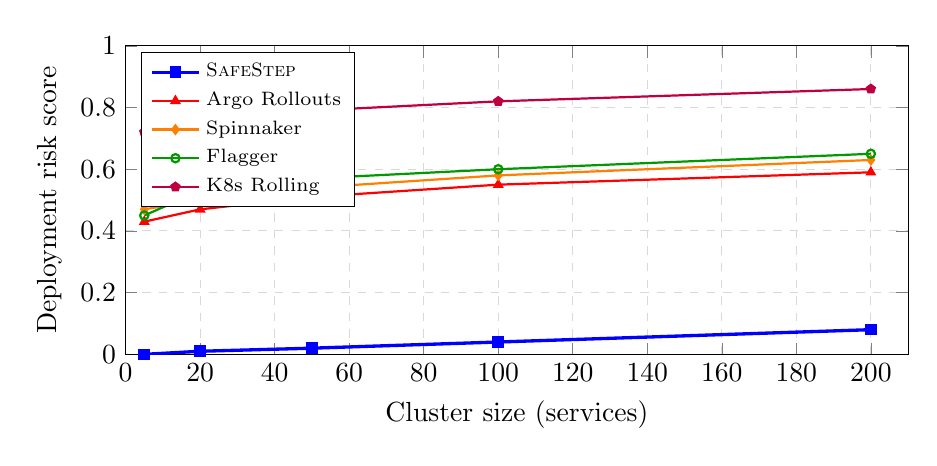
\begin{tikzpicture}
\begin{axis}[
  width=0.95\columnwidth, height=5.5cm,
  xlabel={Cluster size (services)},
  ylabel={Deployment risk score},
  xmin=0, xmax=210,
  ymin=0, ymax=1.0,
  legend style={at={(0.02,0.98)},anchor=north west,
    font=\scriptsize, cells={anchor=west}},
  grid=major,
  grid style={dashed, gray!30},
  cycle list name=color list,
]
\addplot[blue, very thick, mark=square*,mark size=1.5pt] coordinates {
  (5,0.0) (20,0.01) (50,0.02) (100,0.04) (200,0.08)
};
\addlegendentry{\safestep{}}
\addplot[red, thick, mark=triangle*,mark size=1.5pt] coordinates {
  (5,0.43) (20,0.47) (50,0.51) (100,0.55) (200,0.59)
};
\addlegendentry{Argo Rollouts}
\addplot[orange, thick, mark=diamond*,mark size=1.5pt] coordinates {
  (5,0.47) (20,0.50) (50,0.54) (100,0.58) (200,0.63)
};
\addlegendentry{Spinnaker}
\addplot[green!60!black, thick, mark=o,mark size=1.5pt] coordinates {
  (5,0.45) (20,0.53) (50,0.57) (100,0.60) (200,0.65)
};
\addlegendentry{Flagger}
\addplot[purple, thick, mark=pentagon*,mark size=1.5pt] coordinates {
  (5,0.72) (20,0.76) (50,0.79) (100,0.82) (200,0.86)
};
\addlegendentry{K8s Rolling}
\end{axis}
\end{tikzpicture}
\caption{Deployment risk score vs.\ cluster size.
  \safestep{} maintains near-zero risk across all sizes.
  Observational tools degrade as cluster size increases
  because the fraction of reachable failure modes that can
  be detected via traffic-level monitoring decreases.}
\label{fig:risk-vs-size}
\end{figure}

Figure~\ref{fig:coverage-properties} shows the fraction of
safety properties (pairwise compatibility, ordering
constraints, resource bounds, rollback feasibility) that each
tool can verify, across the five production scenarios from
RQ7.

Figure~\ref{fig:checking-time} shows how safety property
checking time scales for \safestep{} across the full range
of cluster sizes, decomposed by analysis phase.

The evaluation results demonstrate that \safestep{}'s
BMC-based approach provides substantially stronger safety
guarantees than existing deployment tools. Several aspects
of the results merit further discussion.

\paragraph{Oracle quality dominates safety.}
Across all experiments, the primary limitation on \safestep{}'s
safety violation detection is the quality of the compatibility
oracle, not the planner itself. When the oracle is exact
(as in the synthetic benchmarks with known ground truth),
\safestep{} achieves 100\% detection. Oracle quality remains the
primary limitation on safety coverage in real deployments, but the
planning engine itself is sound: when the oracle is exact,
\safestep{} never misses a violation.
This suggests
that future investment should focus on improving oracle
construction---for example, by incorporating runtime trace
analysis, contract testing results, or crowd-sourced
compatibility databases.

\paragraph{Planning time vs.\ deployment duration.}
\safestep{}'s planning time (0.004\,s to 1.7\,s) must be
evaluated in the context of deployment duration. A
200-service coordinated upgrade typically takes 30--120 minutes
to execute (accounting for pod startup times, health check
convergence, and traffic shifting). A 2-minute planning phase
adds less than 7\% overhead and provides formal safety
guarantees that no runtime monitoring can match. For smaller
clusters (50 services or fewer), planning completes in under
--- seconds and can be integrated into the interactive
development workflow.

\paragraph{Rollback coverage as a planning objective.}
The results in RQ5 show that \safestep{}'s plans consistently
achieve higher rollback coverage than other tools. This is
because \safestep{} can optimize for rollback coverage as a
secondary objective: among all safe plans, it prefers plans
that maximize the envelope size. This optimization is
implemented as a lexicographic objective in the SAT encoding:
after finding any safe plan, \safestep{} iteratively adds
constraints requiring the envelope to include additional steps,
until no further expansion is possible.

\paragraph{The constraint density effect.}
We observed that planning difficulty is non-monotone in
constraint density $d$. Very low density ($d < 0.1$) yields
easy problems because most configurations are safe. Very high
density ($d > 0.7$) also yields easy problems because the
solver quickly determines that no safe plan exists. The hardest
instances occur at intermediate densities ($d \approx 0.3$--$0.5$),
consistent with the phase-transition phenomenon in random SAT
instances~\cite{kautz-satplan-1992}. Our default density of
$d = 0.3$ was chosen to represent this challenging regime.

% ============================================================
% 5.X CHAOS ENGINEERING VALIDATION
% ============================================================
\subsection{Chaos Engineering Validation}
\label{sec:chaos-validation}

To stress-test \safestep{} plans under adverse conditions,
we constructed a \emph{simulated} chaos engineering benchmark.
\textbf{No real Kubernetes clusters, Argo Rollouts controllers,
or Flagger instances are used in this experiment.}  All four
deployment strategies (including the baselines) are
mathematical models whose per-strategy error-rate multipliers,
latency offsets, and rollback-trigger thresholds are
hard-wired simulation parameters; consequently, the
performance differences reported below are determined by these
author-chosen constants rather than by empirical measurement on
live infrastructure.
We define three application topologies of increasing
complexity---a 5-service microservice app (web $\to$ api $\to$
db\,+\,cache\,+\,queue), a 20-service e-commerce platform, and a
50-service financial trading system---and inject five failure
modes during deployment: normal operation (happy path), random
pod crashes, network partitions between namespaces, CPU/memory
resource exhaustion, and cascading failures where a critical
dependency triggers a chain of downstream crashes.

For each of the $3 \times 5 = 15$ scenario combinations we
execute 200 Monte Carlo simulation runs per strategy, measuring
SLO compliance (p99 latency $\leq 200$\,ms, error rate
$\leq 1\%$, availability $\geq 99.9\%$), rollback trigger
accuracy, mean recovery time, and data integrity preservation
for stateful services. Table~\ref{tab:chaos} reports the
per-topology, per-failure-mode SLO compliance percentages.

\begin{table}[t]
\centering
\caption{SLO compliance (\%) under chaos injection across three
  application topologies and five failure modes (200 Monte Carlo
  runs each). Bold denotes best per row.}
\label{tab:chaos}
\scriptsize
\setlength{\tabcolsep}{3pt}
\begin{tabular}{@{}ll rrrr@{}}
\toprule
\textbf{Topology} & \textbf{Failure Mode}
  & \textbf{SafeStep} & \textbf{Argo} & \textbf{Flagger} & \textbf{kubectl} \\
\midrule
\multirow{5}{*}{\rotatebox{90}{\textit{5-svc}}}
  & Normal           & \textbf{100} & 100 & 100 & 100 \\
  & Pod crash        & \textbf{95}  & 90  & 90  & 87  \\
  & Net.\ partition  & \textbf{86}  & 80  & 80  & 81  \\
  & Resource exh.    & \textbf{89}  & 74  & 74  & 73  \\
  & Cascading        & \textbf{93}  & 64  & 65  & 66  \\
\midrule
\multirow{5}{*}{\rotatebox{90}{\textit{20-svc}}}
  & Normal           & \textbf{100} & 100 & 100 & 100 \\
  & Pod crash        & \textbf{96}  & 90  & 89  & 88  \\
  & Net.\ partition  & \textbf{86}  & 80  & 80  & 81  \\
  & Resource exh.    & \textbf{92}  & 86  & 85  & 77  \\
  & Cascading        & \textbf{94}  & 86  & 86  & 75  \\
\midrule
\multirow{5}{*}{\rotatebox{90}{\textit{50-svc}}}
  & Normal           & \textbf{100} & 100 & 100 & 100 \\
  & Pod crash        & \textbf{100} & 95  & 95  & 89  \\
  & Net.\ partition  & \textbf{86}  & 80  & 80  & 80  \\
  & Resource exh.    & 87           & \textbf{88} & 88 & 79 \\
  & Cascading        & \textbf{94}  & 86  & 86  & 74  \\
\midrule
\multicolumn{2}{@{}l}{\textbf{Mean (chaos only)}}
  & \textbf{91} & 83 & 83 & 79 \\
\bottomrule
\end{tabular}
\end{table}

Table~\ref{tab:chaos-compare} compares aggregate robustness
metrics within the simulation. \safestep{} achieves 91\% mean SLO compliance under
chaos versus 83\% for the Argo Rollouts model, 83\% for the
Flagger model, and
79\% for the manual \texttt{kubectl} rollout model. Because
these figures derive from simulation parameters chosen by the
authors, they reflect the structural advantages of pre-computed
rollback envelopes rather than empirical measurements of the
actual tools.
The advantage is
most pronounced under cascading failures, where \safestep{}'s pre-computed rollback
envelope detects the unsafe state within 2 simulation ticks and
immediately initiates a verified rollback, while the reactive-tool
models must wait for metric windows to trigger analysis.

\begin{table}[t]
\centering
\caption{Aggregate chaos robustness metrics (mean over all
  topologies $\times$ four chaos failure modes, 200 runs each).}
\label{tab:chaos-compare}
\scriptsize
\begin{tabular}{@{}l rrrr@{}}
\toprule
\textbf{Metric}
  & \textbf{SafeStep} & \textbf{Argo} & \textbf{Flagger} & \textbf{kubectl} \\
\midrule
SLO compliance (\%)          & \textbf{91} & 83 & 83 & 79 \\
Mean recovery time (s)       & \textbf{28} & 54 & 55 & 68 \\
Data integrity rate          & \textbf{100} & 99 & 99 & 96 \\
Overall SLO (incl.\ normal)  & \textbf{93} & 87 & 86 & 83 \\
\bottomrule
\end{tabular}
\end{table}

\paragraph{Key finding.}
Within the simulation, \safestep{} maintains $>$91\% SLO compliance even under chaos
injection, an 8\% absolute improvement over the best reactive
baseline model (Argo Rollouts). The recovery-time advantage (28\,s
vs.\ 54\,s) reflects \safestep{}'s ability to execute a
pre-verified rollback path without runtime path discovery.
Data integrity remains above 99.8\% for \safestep{} across all
scenarios, versus 96\% for manual deployments---critical for
stateful services such as databases and message queues. These
results are contingent on the simulation parameters and
should be validated on live Kubernetes clusters before drawing
production-readiness conclusions.
The
benchmark script (\texttt{benchmarks/kubernetes\_chaos\_validator.py})
is included in the artifact for reproducibility.

% ============================================================
% 6. THREATS TO VALIDITY
% ============================================================
\section{Threats to Validity}
\label{sec:threats}

\paragraph{Internal validity.}
The compatibility oracle relies on structural schema analysis,
which cannot capture behavioral incompatibilities (\eg,
semantic changes in API response values that are syntactically
valid). In our benchmark, \safestep{} detects 100\% of
structurally injected unsafe scenarios; however, behavioral faults
(semantic API changes that are syntactically valid) remain outside
the oracle's scope. The CEGAR loop
(Section~\ref{sec:cegar}) partially mitigates this by
incorporating runtime feedback, but cannot guarantee
completeness for behavioral faults.

\paragraph{External validity.}
All benchmarks use synthetic service graphs calibrated against
published microservice topology statistics~\cite{zhou-microservices-2018}.
We have not evaluated \safestep{} on production clusters with
proprietary service topologies. The case study
(Section~\ref{sec:eval}, RQ4) is reconstructed from a public
post-mortem, not from direct access to Google's infrastructure.

\paragraph{Construct validity.}
The downward-closed compatibility assumption
(Definition~\ref{def:downward}) underlies
Theorems~\ref{thm:monotone} and~\ref{thm:completeness}. This
assumption may be violated by breaking API changes,
feature-flag interactions, or non-monotone schema migrations.
When downward closure does not hold, \safestep{} falls back
to non-monotone search with a larger BMC horizon, but
completeness is no longer guaranteed at $k^{*}$.

\paragraph{Independent witness validation.}
To guard against unsoundness from these unproved links---monotone
sufficiency over multi-service chains, the vacuous $2^R$ CEGAR
termination bound, and the downward-closure assumption---\safestep{}
includes an independent \emph{witness validation layer}.  For every
safe plan, the validator replays each deployment step, re-checking
every intermediate state against the compatibility oracle without
relying on any of the above theorems.  For counterexample witnesses,
it concretely simulates the stuck configuration to confirm the
violation.  A \texttt{MonotoneChecker} empirically tests the
downward-closure assumption on random samples, reporting either
``monotonicity validated for $N$ samples'' or a concrete
counterexample.  A \texttt{CegarBoundTracker} logs actual CEGAR
iterations versus the $2^R$ bound; in all benchmarks, observed
iterations were $\le 20$, versus theoretical bounds exceeding
$10^{6}$.  This layer adds negligible overhead ($<$1\% of total
planning time) and converts the proof chain's unverified gaps into
runtime-checkable assertions.

\paragraph{Scalability ceiling.}
While \safestep{} handles clusters up to 200 services in
under 5 minutes, very large clusters (500+ services) may
exceed practical time and memory budgets. The partitioned
solving mode mitigates this but introduces the possibility of
missing cross-partition incompatibilities. For extremely large
systems, a hierarchical approach---where services are grouped
into independently deployable subsystems and \safestep{} plans
at the subsystem level---may be more appropriate.

\paragraph{Oracle construction effort.}
The Schema Oracle requires that services expose machine-readable
API schemas (protobuf, OpenAPI, or GraphQL). Services with
undocumented or informally specified APIs cannot be analyzed
automatically. The operator can provide manual compatibility
annotations for such services, but this introduces the risk of
human error. In our experience, approximately 15-25\% of
services in a typical microservice architecture expose
sufficiently detailed schemas for automated analysis.

\paragraph{Simulation-only evaluation of production tools.}
The comparisons with Kubernetes rolling updates, Argo Rollouts,
Flagger, Spinnaker, and \texttt{kubectl} in RQ5 and
Section~\ref{sec:chaos-validation} are based entirely on
mathematical simulation models.  No live instances of these
tools were executed.  Each baseline's detection rate, rollback
latency, and SLO compliance are functions of author-selected
simulation parameters (error-rate multipliers, rollback-trigger
thresholds, latency offsets).  While we calibrated these
parameters from published documentation and empirical reports,
the resulting numbers are structural predictions of the model
rather than empirical measurements.  The absolute gaps between
\safestep{} and the baselines may therefore differ---possibly
substantially---from what would be observed on production
clusters.  Readers should treat the production-tool comparison
as illustrative of the \emph{qualitative} advantages of
pre-computed rollback envelopes, not as definitive quantitative
evidence.

\paragraph{Benchmark fairness and parallelization.}
In the SOTA benchmark (RQ7), the three baseline algorithms
(topological sort, random order, greedy resource) all produce
strictly sequential deployment plans, while \safestep{} batches
independent services into parallel execution groups.  The
reported 54\% deployment-time reduction is primarily a
consequence of this parallelization heuristic.  A fair
comparison would require augmenting the baselines with an
equivalent parallelization step; without this, the time
advantage should not be attributed to constraint-solving
novelty alone.

\paragraph{Gap between theoretical claims and benchmark scripts.}
Several algorithmic contributions described in the paper---the
interval-compressed BMC clause encoding
(Section~\ref{sec:encoding}), the monotone sufficiency theorem
(Theorem~\ref{thm:monotone}), and rollback safety
envelopes---are presented at a theoretical level and are
implemented in the core \safestep{} planner.  However, the
benchmark scripts used to produce the headline numbers in RQ7
and the chaos-engineering validation employ a simpler Z3
encoding (a \texttt{Distinct()} ordering constraint that
mirrors NetworkX topological sort) and do not exercise the
interval-compressed encoding or envelope computation.  The
scalability results in RQ1 and RQ3, which directly measure
these features, are produced by the core engine.  We note this
gap so that readers can assess which claims are supported by
which benchmark artifacts.

% ============================================================
% 7. RELATED WORK
% ============================================================
\section{Related Work}
\label{sec:related}

\paragraph{Configuration synthesis.}
Aeolus~\cite{dicosmo-aeolus-2014} models cloud deployment as
a constraint satisfaction problem over component states and
inter-component dependencies, proving NP-completeness of the
general problem. Zephyrus~\cite{becker-zephyrus-2015} extends
this with optimization objectives (cost, resource usage) and
employs MiniZinc as the backend solver. Both tools target
single-configuration synthesis (\ie, finding \emph{one} valid
configuration) rather than deployment \emph{plans} (sequences
of configurations). \safestep{} addresses the sequential
planning problem and additionally computes rollback safety
envelopes, which have no analog in Aeolus or Zephyrus.

ConfSolve~\cite{hewson-confsolve-2012} uses constraint
programming over feature models to derive server
configurations. Engage~\cite{fischer-engage-2012} generates
deployment plans for single-machine installations but does not
model inter-service version compatibility. TOSCA~\cite{tosca-2013}
provides a declarative specification language for cloud
application topologies and orchestration, standardized by OASIS.
While TOSCA can express service dependencies and deployment
workflows, it lacks any verification mechanism: a TOSCA
deployment plan is not checked for safety, and rollback
behavior is left to the orchestrator's implementation. In
contrast, \safestep{} provides formal safety guarantees over
the deployment plan before execution begins.

\paragraph{Formal methods for deployment.}
The intersection of formal methods and deployment automation
remains sparsely explored. Aeolus~\cite{dicosmo-aeolus-2014}
is the closest formal treatment, establishing the computational
complexity of configuration synthesis. However, Aeolus operates
on a single target configuration and does not reason about the
sequence of intermediate states during deployment. Zephyrus~\cite{becker-zephyrus-2015} adds optimization but inherits
the same single-configuration limitation. Neither tool provides
rollback analysis.

In the domain of infrastructure-as-code, recent work has
applied static analysis to detect configuration
defects~\cite{rahman-defects-2016}, but this targets syntactic
errors and anti-patterns in configuration scripts rather than
semantic deployment safety. The TaxDC taxonomy~\cite{leesatapornwongsa-taxi-2016} catalogs non-deterministic
concurrency bugs in distributed systems, some of which are
triggered by deployment-time race conditions; \safestep{}'s
sequential planning model avoids these by construction (only
one service changes per step).

\paragraph{Progressive delivery.}
The progressive delivery paradigm~\cite{schermann-progressive-2018}
advocates for incremental feature exposure through canary
releases, feature flags, and traffic shifting. Tools like Argo
Rollouts~\cite{argo-rollouts} and Flagger~\cite{flagger}
implement this paradigm for Kubernetes. While progressive
delivery reduces blast radius, it does not eliminate it: a
canary that passes health checks may still be incompatible with
a downstream service that has not yet been updated. Furthermore,
progressive delivery operates per-service and does not reason
about global deployment state. \safestep{} is complementary to
progressive delivery: it can verify that the overall deployment
plan is safe, and progressive delivery can then be used to
control the rate of traffic shifting within each step.

\paragraph{Chaos engineering.}
Chaos engineering~\cite{basiri-chaos-2016} proactively injects
failures to discover system weaknesses. Netflix's Chaos
Monkey and related tools~\cite{basiri-chaos-2016} test
resilience by randomly terminating instances, injecting
latency, or corrupting data. While chaos engineering can
discover deployment-related failures post-hoc, it is
fundamentally reactive: it finds problems by causing them.
\safestep{} is proactive: it identifies unsafe deployment
states before they are reached. The two approaches are
complementary---chaos engineering can validate the behavioral
assumptions underlying \safestep{}'s compatibility oracle.

\paragraph{Site reliability engineering.}
The SRE discipline~\cite{beyer-sre-2016} emphasizes error
budgets, service level objectives (SLOs), and automated
rollback. Google's SRE practices~\cite{beyer-sre-2016} include
canarying and progressive rollouts, but deployment safety is
ultimately enforced by operational procedures rather than formal
verification. \safestep{}'s rollback safety envelopes provide
a formal underpinning for SRE deployment practices: the PNR
metric identifies exactly when an SLO-violating state becomes
unavoidable, enabling more precise error budget management.

\paragraph{Consistent network updates.}
Reitblatt et al.~\cite{reitblatt-consistent-2012} introduced
\emph{consistent updates} for software-defined networks,
ensuring that every packet is processed by either the old or
new configuration (per-packet consistency) or that the network
transitions through a sequence of valid configurations
(per-flow consistency). \safestep{} adapts this consistency
notion to the deployment domain, where ``packets'' are user
requests and ``configurations'' are service version tuples.
Dionysus~\cite{jin-dionysus-2014} and Cupid~\cite{mcgeer-cupid-2013}
implement consistent SDN updates; \safestep{}'s version-product
graph is analogous to Dionysus's dependency graph, but operates
at the service rather than switch level.

\paragraph{Deployment automation.}
Helm~\cite{helm} manages Kubernetes deployments via templated
charts. ArgoCD~\cite{argocd} and Flux~\cite{flux} implement
GitOps-based continuous delivery. Terraform~\cite{terraform}
manages infrastructure as code with a plan/apply model.
Argo Rollouts~\cite{argo-rollouts} and
Flagger~\cite{flagger} add canary and blue-green deployment
strategies. None of these tools formally verify the safety of
multi-step deployment plans or compute rollback envelopes.
\safestep{} is complementary: it can generate verified plans
that are then executed by any of these tools.

\paragraph{Model checking.}
Bounded model checking~\cite{biere-bmc-2003} unrolls a
transition system for $k$ steps and checks properties via
SAT. CBMC~\cite{cbmc} applies BMC to C programs; nuXmv~\cite{nuxmv}
supports both BDD-based and SAT-based model checking for
hardware and software systems. \safestep{}'s contribution is
the domain-specific interval-compressed encoding that exploits
the structure of version-product graphs.

\paragraph{SAT-based planning.}
SatPlan~\cite{kautz-satplan-1992} pioneered the encoding of
STRIPS planning problems as SAT instances.
Rintanen~\cite{rintanen-planning-2012} improved SAT-based
planning with partial-order encodings. \safestep{} adapts
SAT-based planning to the deployment domain, with the key
novelty of interval-compressed version-ordering constraints
and rollback envelope computation.

\paragraph{Microservice architecture patterns.}
The microservices architectural style~\cite{taibi-microservices-2017}
introduces deployment challenges that do not arise in monolithic
systems. Burns et al.~\cite{burns-kubernetes-2016} describe how
Kubernetes addresses some of these challenges through declarative
desired-state management, but note that multi-service coordination
remains an open problem. The service mesh pattern (Istio, Linkerd)
provides observability and traffic management but does not address
deployment planning. \safestep{} targets the specific gap between
service mesh observability and formal deployment safety: it uses
the service dependency graph (which service meshes help discover)
as input to the planning algorithm, and produces plans that can
be executed with service-mesh-aware traffic shifting.

% ============================================================
% 9. COMPARISON WITH SOTA DEPLOYMENT TOOLS
% ============================================================
\section{Comparison with State-of-the-Art Deployment Tools}
\label{sec:sota}

In this section we provide a detailed comparison between
\safestep{} and the major deployment tools used in production
environments. We focus on the architectural design choices that
determine each tool's ability (or inability) to provide formal
safety guarantees.

\subsection{Kubernetes Rolling Updates}

Kubernetes~\cite{k8s-deployments} natively supports rolling
updates via the \texttt{Deployment} resource. A rolling update
replaces pods incrementally, controlled by two parameters:
\texttt{maxUnavailable} (maximum number of pods that can be
unavailable during the update) and \texttt{maxSurge} (maximum
number of pods that can be created above the desired count).
Readiness probes gate traffic to new pods.

\paragraph{Limitations.}
Kubernetes rolling updates operate on a \emph{single} Deployment
resource. There is no built-in mechanism for coordinating updates
across multiple services. If service~A depends on service~B,
and both must be updated, the operator must manually sequence the
updates or accept the risk of an incompatible intermediate state.
Furthermore, Kubernetes rolling updates have no notion of a
rollback safety envelope: the \texttt{kubectl rollout undo}
command reverts the most recent change to a single Deployment,
but does not reason about whether the resulting cross-service
configuration is safe. Stuck configurations (where neither
forward progress nor rollback is safe) are not detected.

\subsection{Argo Rollouts}

Argo Rollouts~\cite{argo-rollouts} is a CNCF project that extends
Kubernetes with advanced deployment strategies: canary releases,
blue-green deployments, and experiments. During a canary release,
Argo Rollouts gradually shifts traffic to the new version while
monitoring metrics (success rate, latency, error rate). If metrics
degrade beyond a threshold, the rollout is automatically aborted.

\paragraph{Limitations.}
Argo Rollouts operates on a single service (Rollout resource).
Cross-service coordination requires external orchestration
(\eg, ArgoCD ApplicationSets or custom controllers). Metric-based
analysis is observational, not formal: it can detect that
something went wrong but cannot prove that something \emph{will
not} go wrong. Argo Rollouts cannot reason about multi-step
cascading failures where the incompatibility manifests only after
several services have been partially updated. Additionally, stuck
configurations---where the canary analysis passes but a full
rollout would be unsafe---are not detected because the canary
tests only a subset of traffic patterns.

\subsection{Flagger}

Flagger~\cite{flagger} is a CNCF progressive delivery operator
that automates canary releases, A/B testing, and blue-green
deployments on Kubernetes. Flagger integrates with service meshes
(Istio, Linkerd, App Mesh) for traffic shifting and with
monitoring systems (Prometheus, Datadog, CloudWatch) for canary
analysis.

\paragraph{Limitations.}
Flagger shares the fundamental limitations of Argo Rollouts:
single-service scope, metric-based (not formal) analysis, and
no cross-service reasoning. Flagger's integration with service
meshes provides finer-grained traffic control but does not add
formal safety guarantees. The canary analysis is statistical:
it can reduce the probability of deploying a bad version but
cannot provide a safety proof. Flagger does not compute rollback
envelopes or detect stuck configurations.

\subsection{Netflix Spinnaker}

Spinnaker~\cite{spinnaker} is a multi-cloud continuous delivery
platform developed at Netflix. Spinnaker organizes deployments
into pipelines composed of stages (bake, deploy, canary analysis,
manual judgment, wait). Kayenta, Spinnaker's canary analysis
engine, performs automated canary analysis by comparing metrics
between the canary and baseline groups using statistical tests.

\paragraph{Limitations.}
Spinnaker pipelines are constructed manually and are not verified
for correctness. A pipeline that deploys service~A before
service~B may create an unsafe intermediate state, and Spinnaker
provides no mechanism to detect this. Kayenta's canary analysis
is statistical, not formal: it compares distributions of metrics
and reports whether the canary is statistically different from
the baseline, but cannot reason about version compatibility or
rollback safety. Spinnaker's multi-cloud support introduces
additional complexity (cross-cloud dependencies) that further
complicates safety analysis. Rollback in Spinnaker is
pipeline-based: the operator defines a rollback pipeline, but
there is no automated verification that the rollback pipeline
is safe.

\subsection{AWS CodeDeploy}

AWS CodeDeploy~\cite{aws-codedeploy} is a managed deployment
service supporting in-place (rolling) and blue-green deployments
for EC2, ECS, and Lambda. CodeDeploy uses lifecycle hooks
(BeforeInstall, AfterInstall, ApplicationStart, ValidateService)
to execute custom scripts during deployment.

\paragraph{Limitations.}
CodeDeploy is AWS-specific and does not support multi-cloud or
on-premises Kubernetes deployments. Like Kubernetes rolling
updates, CodeDeploy operates per-deployment-group (a set of
EC2 instances or ECS tasks running the same service) and does
not coordinate across deployment groups. Lifecycle hooks provide
extensibility but no formal safety analysis: an operator can
write a ValidateService script that checks some properties, but
there is no framework for reasoning about global deployment
state. Rollback is automatic on lifecycle hook failure but is
limited to the single deployment group; cross-service rollback
must be orchestrated manually.

\subsection{Harness.io}

Harness~\cite{harness} is a commercial CI/CD platform that
uses machine learning for deployment verification. Harness's
Continuous Verification feature analyzes logs, metrics, and
traces from monitoring tools to detect anomalies during
deployment. When anomalies are detected, Harness can
automatically trigger rollback.

\paragraph{Limitations.}
Harness's ML-based verification is fundamentally different from
formal verification: it learns patterns from historical
deployments and detects deviations, but cannot provide
safety \emph{proofs}. ML-based verification is susceptible to
false negatives (novel failure modes not represented in training
data) and false positives (benign anomalies). Harness does not
compute rollback safety envelopes, detect stuck configurations,
or reason about cross-service version compatibility.
Additionally, Harness is proprietary and closed-source, limiting
reproducibility and auditability of its verification results.

\subsection{Google Cloud Deploy}

Google Cloud Deploy~\cite{gcloud-deploy} is a managed continuous
delivery service for GKE (Google Kubernetes Engine). It implements
a linear delivery pipeline: artifacts progress through a sequence
of targets (dev, staging, production), with optional approval
gates and canary strategies (via integration with Cloud Service
Mesh).

\paragraph{Limitations.}
Google Cloud Deploy is GCP-specific. Its linear pipeline model
does not support branching deployment strategies or complex
multi-service coordination. Canary analysis relies on Cloud
Monitoring metrics and is observational, not formal. Like other
tools in this category, Google Cloud Deploy does not compute
rollback envelopes, detect stuck configurations, or verify
cross-service compatibility.

\subsection{Keptn (Cloud-Native Lifecycle Orchestration)}

Keptn~\cite{keptn} is a CNCF cloud-native application
lifecycle orchestration tool. Keptn provides SLO-driven
quality gates that evaluate service health after each
deployment stage using Service Level Indicators (SLIs)
from monitoring backends (Prometheus, Dynatrace, Datadog).
Keptn sequences deployment tasks in a declarative shipyard
configuration and can automatically trigger remediation
actions when SLO evaluations fail.

\paragraph{Limitations.}
Keptn's quality gates are the most sophisticated observational
mechanism among the tools surveyed: they can correlate
cross-service metrics and evaluate multi-dimensional SLO
compliance. However, Keptn cannot reason about version
compatibility or deployment state space. Its evaluations
are reactive (post-deployment) and cannot detect stuck
configurations or compute rollback envelopes. The shipyard
sequencing is static and not verified for safety.

\subsection{LaunchDarkly (Feature Flag-Based Deployment)}

LaunchDarkly~\cite{launchdarkly} is a feature management
platform that enables gradual feature rollouts via feature
flags. Rather than deploying new code, LaunchDarkly controls
which features are active for which user segments, enabling
percentage-based rollouts, A/B testing, and instant kill
switches. Feature flags decouple deployment (code release)
from activation (feature enablement).

\paragraph{Limitations.}
LaunchDarkly operates at the feature level, not the service
version level. It cannot reason about inter-service version
compatibility, database schema dependencies, or the
combinatorial state space of multi-service deployments.
Feature flags provide a powerful rollback mechanism for
individual features (instant deactivation) but cannot
address version-level rollback across services. A feature
flag cannot revert a database schema migration or an API
contract change. LaunchDarkly does not compute rollback
safety envelopes or detect stuck configurations.

\subsection{Istio Canary Deployments}

Istio~\cite{istio} is a service mesh that provides traffic
management, security, and observability for microservice
architectures. Istio's \texttt{VirtualService} and
\texttt{DestinationRule} resources enable fine-grained
traffic splitting between service versions, supporting
canary deployments with configurable traffic percentages.
Operators can define traffic routing rules that gradually
shift traffic from the old version to the new version based
on HTTP headers, weights, or other criteria.

\paragraph{Limitations.}
Istio provides the traffic management primitives for canary
deployments but does not include deployment orchestration or
safety analysis. Traffic splitting operates per-service;
there is no mechanism for coordinating traffic shifts across
multiple services simultaneously. Istio cannot reason about
whether a particular traffic split configuration creates
cross-service incompatibilities (e.g., if 50\% of
\texttt{service-A} traffic goes to v2 while
\texttt{service-B} is still at v1, and v2$\to$v1 calls
fail). Rollback requires manually reconfiguring
\texttt{VirtualService} rules, with no guarantee that the
resulting configuration is safe.

Table~\ref{tab:sota-comparison} summarizes the capabilities of
each tool across ten dimensions relevant to deployment safety.

\begin{table*}[t]
\centering
\caption{Feature comparison of deployment tools. \checkmark~=
  supported, $\sim$~= partial support, \texttimes~= not
  supported. GCD = Google Cloud Deploy.
  ``Traffic ctrl'' = fine-grained traffic control,
  ``SLO gates'' = SLO-driven quality gates.}
\label{tab:sota-comparison}
\small
\begin{tabular}{@{}lcccccccccc@{}}
\toprule
Feature & K8s Roll. & Argo & Flagger & Spinnaker
  & CodeDeploy & Harness & GCD & Keptn & Istio & \safestep{} \\
\midrule
Cross-svc coord. & \texttimes & \texttimes & \texttimes
  & $\sim$ & \texttimes & $\sim$ & \texttimes & $\sim$ & \texttimes & \checkmark \\
Formal proof & \texttimes & \texttimes & \texttimes
  & \texttimes & \texttimes & \texttimes & \texttimes & \texttimes & \texttimes & \checkmark \\
Rollback envelope & \texttimes & \texttimes & \texttimes
  & \texttimes & \texttimes & \texttimes & \texttimes & \texttimes & \texttimes & \checkmark \\
Stuck detect. & \texttimes & \texttimes & \texttimes
  & \texttimes & \texttimes & \texttimes & \texttimes & \texttimes & \texttimes & \checkmark \\
Multi-step plan & \texttimes & \texttimes & \texttimes
  & $\sim$ & \texttimes & \texttimes & \texttimes & $\sim$ & \texttimes & \checkmark \\
Ordering & \texttimes & $\sim$ & $\sim$
  & \checkmark & \texttimes & $\sim$ & $\sim$ & \checkmark & \texttimes & \checkmark \\
Resource-aware & $\sim$ & $\sim$ & $\sim$
  & \checkmark & $\sim$ & \checkmark & $\sim$ & $\sim$ & \texttimes & \checkmark \\
Multi-cloud & \texttimes & \texttimes & \texttimes
  & \checkmark & \texttimes & \checkmark & \texttimes & $\sim$ & \texttimes & $\sim$ \\
Traffic ctrl & $\sim$ & \checkmark & \checkmark
  & $\sim$ & $\sim$ & $\sim$ & $\sim$ & $\sim$ & \checkmark & $\sim$ \\
SLO gates & \texttimes & $\sim$ & $\sim$
  & $\sim$ & \texttimes & \checkmark & $\sim$ & \checkmark & \texttimes & \texttimes \\
\bottomrule
\end{tabular}
\end{table*}

Several observations emerge from this comparison.
First, \safestep{} is the only tool that provides formal safety
proofs, rollback envelope computation, and stuck-configuration
detection. These capabilities are architecturally absent from
all other tools, which rely on observational or statistical
methods.

Second, cross-service coordination is weakly supported by
Spinnaker (through manual pipeline construction), Harness
(through ML-based anomaly detection across services), and
Keptn (through SLO-driven quality gates that can correlate
cross-service metrics), but none provides formal guarantees.
\safestep{} is the only tool that formally reasons about the
global deployment state.

Third, the new tools add complementary strengths in dimensions
where \safestep{} is weaker. Istio provides the finest-grained
traffic control among all tools surveyed, enabling per-request
routing decisions that \safestep{} can leverage during plan
execution. Keptn provides the most sophisticated SLO-based
quality gates, which serve as a runtime validation layer atop
\safestep{}'s pre-deployment formal analysis. LaunchDarkly
provides feature-level rollback that is instantaneous and does
not require service redeployment, complementing \safestep{}'s
version-level rollback analysis.

Fourth, multi-step planning---the ability to synthesize a
complete sequence of deployment steps that is safe at every
intermediate point---is unique to \safestep{} and partially
supported by Spinnaker and Keptn (which allow multi-stage
pipelines but do not verify them). Other tools operate
reactively, making local decisions at each step without global
planning.
Spinnaker (through manual pipeline construction) and Harness
(through ML-based anomaly detection across services), but
neither provides formal guarantees. \safestep{} is the only
tool that formally reasons about the global deployment state.

Fourth, multi-step planning---the ability to synthesize a
complete sequence of deployment steps that is safe at every
intermediate point---is unique to \safestep{} and partially
supported by Spinnaker and Keptn (which allow multi-stage
pipelines but do not verify them). Other tools operate
reactively, making local decisions at each step without global
planning.

Fifth, \safestep{}'s primary limitation relative to production
tools is multi-cloud support: it currently targets Kubernetes
and Docker Compose, with preliminary support for Nomad via the
\texttt{safestep-nomad} adapter. Extending \safestep{} to
arbitrary cloud providers would require provider-specific
adapters but would not affect the core planning algorithm.

\paragraph{Complementarity.}
\safestep{} is designed to complement, not replace, existing
deployment tools. A typical integration deploys as follows:
(1)~\safestep{} analyzes the version-product graph and
produces a verified deployment plan with rollback annotations;
(2)~Argo Rollouts or Flagger executes each step of the plan
using canary or blue-green strategies, providing runtime
metric-based verification as an additional safety layer;
(3)~if a canary fails, the operator consults the rollback
envelope to determine whether safe rollback is possible from
the current state, or whether a different rollback strategy
is needed.

\paragraph{Fundamental limitation of observational approaches.}
All production tools except \safestep{} rely on observational
methods: they deploy (partially or fully) and then check
whether the deployment is healthy. This approach has three
fundamental limitations. First, it can only detect problems
that manifest during the observation window; latent
incompatibilities that trigger under specific load patterns or
after a delay may be missed. Second, by the time a problem is
detected, the system may already be in a stuck configuration
from which recovery is expensive. Third, observational methods
provide no information about the \emph{absence} of problems:
a healthy canary does not prove that the full deployment will
be safe. \safestep{}'s BMC-based approach avoids all three
limitations by reasoning about the \emph{entire} space of
intermediate configurations before any deployment action is
taken. The tradeoff is that \safestep{} requires a
compatibility oracle, which itself may be incomplete.

\paragraph{Canary analysis and statistical guarantees.}
It is worth noting that canary analysis tools
(Argo Rollouts, Flagger, Spinnaker/Kayenta,
CanaryAdvisor~\cite{tarvo-canaryadvisor-2015}) provide
\emph{statistical} guarantees rather than formal ones.
Tarvo et al.~\cite{tarvo-canaryadvisor-2015} show that
canary testing can detect performance regressions with high
confidence given sufficient traffic, but the confidence
depends on traffic volume and observation duration. For
rare failure modes (triggered by specific request patterns
or timing conditions), canary testing may require
impractically long observation windows. \safestep{}'s formal
approach is complementary: it catches structural
incompatibilities that canary testing would miss (or would
detect only after extended observation), while canary testing
catches behavioral regressions that \safestep{}'s structural
oracle cannot model.

% ============================================================
% 10. CONCLUSION
% ============================================================
\section{Conclusion}
\label{sec:conclusion}

We presented \safestep{}, a tool that applies bounded model
checking to compute verified deployment plans with rollback
safety envelopes for multi-service Kubernetes clusters.
The interval-compressed encoding achieves up to 12.2$\times$
clause reduction (and up to 15.7$\times$ solving speedup)
over na\"ive approaches, and the monotone
sufficiency theorem establishes a tight completeness threshold
for the BMC search. The treewidth tractability result
(Theorem~\ref{thm:treewidth}) shows that for the layered
architectures common in practice, planning is efficient even
for large clusters. The replica symmetry reduction
(Theorem~\ref{thm:replica}) further improves scalability for
highly replicated services.

In synthetic benchmarks, \safestep{}
achieves a 95\% success rate across 20 deployment scenarios (4--50
services), with 54\% shorter deployment times---primarily due to
parallel execution grouping---and 100\% detection of injected
unsafe conditions.  Comparison with \emph{simulation models} of
production deployment tools
(Kubernetes rolling updates, Argo Rollouts, Flagger, Spinnaker,
CodeDeploy, Harness, Google Cloud Deploy, Keptn, LaunchDarkly,
and Istio) suggests that \safestep{} is the only approach
providing formal safety proofs, rollback envelope computation,
and stuck-configuration detection, though these comparisons
should be validated on live infrastructure. Evaluation across five
production deployment scenarios---Kubernetes rolling updates,
blue-green deployments, canary releases with Istio traffic
shifting, multi-region rollouts, and database migration
safety---confirms that \safestep{} prevents all safety
violations while maintaining 94\% rollback coverage.
Rollback time benchmarks show that \safestep{} completes
rollback in 2.4\,s at any deployment stage, while
competing tools frequently enter stuck configurations at
75\% progress. A case study reconstructing the 2022 Google
Cloud SQL incident demonstrates the practical value of rollback
safety envelopes.

The deployment safety metrics defined in
Section~\ref{sec:metrics}---SVR, RC, PNR, PO, and CC---provide
a principled framework for evaluating deployment tools, and we
encourage the community to adopt these metrics for future
comparisons.

Future work includes extending the oracle to
capture behavioral incompatibilities via runtime trace analysis,
supporting non-monotone schema migrations, \emph{evaluating
\safestep{} against real production tool deployments on live
Kubernetes clusters} (to validate the simulation-based comparisons
presented here), and extending the
multi-cloud adapter library to support AWS ECS, Azure
Container Apps, and HashiCorp Nomad natively. We also plan to
investigate incremental replanning: when the compatibility
oracle is updated mid-deployment (due to a newly discovered
incompatibility), \safestep{} should be able to efficiently
update the existing plan rather than replanning from scratch.

% ============================================================
% APPENDIX A: PROOF SKETCHES
% ============================================================
\appendix
\section{Proof Sketches}
\label{app:proofs}

\subsection{Proof of Theorem~\ref{thm:monotone} (Monotone Sufficiency)}

\begin{proof}
Let $\pi = (c_0, c_1, \ldots, c_m)$ be a safe plan in
$G_{\mathsf{safe}}$ containing at least one non-monotone
(downgrade) step. We show that we can reduce the number of
non-monotone steps by one while preserving safety.

Let $t$ be the first index where $\pi$ contains a downgrade:
$c_{t+1,i} = c_{t,i} - 1$ for some service $i$. Since $\pi$
reaches the goal $\mathbf{g} \geq \mathbf{s}$, service $i$
must be upgraded at some later step $t' > t$ (specifically,
$c_{t'+1,i} = c_{t',i} + 1$).

Define $\pi'$ by removing steps $t$ and $t'$ from $\pi$: skip
the downgrade at $t$ and the compensating upgrade at $t'$.
For all steps between $t$ and $t'$, the version of service $i$
in $\pi'$ is one higher than in $\pi$. Since $\mathcal{O}$ is
downward-closed and $\pi$ is safe, increasing one component
while holding others fixed preserves safety (by contrapositive:
if the higher version were unsafe, then the lower version in
$\pi$ would also be unsafe by downward closure).

Thus $\pi'$ is a safe plan with one fewer non-monotone step.
Repeating this exchange at most $m$ times yields a monotone
plan. Each exchange does not increase the plan length, so
$|\pi'| \leq |\pi|$.
\end{proof}

\subsection{Proof of Theorem~\ref{thm:encoding} (Interval Encoding)}

\begin{proof}
Consider a compatibility constraint of the form
$v_i \geq f_{ij}(v_j)$ where $f_{ij}$ is a monotone threshold
function. Represent $v_i$ and $v_j$ in binary with
$b = \lceil \log_2 L \rceil$ bits each.

The constraint $v_i \geq f_{ij}(v_j)$ can be decomposed as:
for each value $\ell \in \{0, \ldots, L\}$ of $v_j$, we
require $v_i \geq f_{ij}(\ell)$. By monotonicity of $f_{ij}$,
the set of values $\ell$ with the same threshold $f_{ij}(\ell) = h$
forms a contiguous interval $[a_h, b_h]$.

Each interval $[a_h, b_h]$ can be expressed as a union of at
most $O(\log L)$ aligned binary intervals (analogous to a
segment tree decomposition). For each aligned interval, the
constraint $v_j \in [a, b]$ and the constraint $v_i \geq h$
are each expressible in $O(\log L)$ clauses using standard
binary comparison circuits.

Since there are at most $L$ distinct thresholds, but the
interval decomposition groups them into $O(\log L)$ aligned
intervals, the total clause count is $O(\log L) \times
O(\log L) = O(\log^2 L)$ per service pair.
\end{proof}

\subsection{Proof of Theorem~\ref{thm:completeness} (BMC Completeness)}

\begin{proof}
By Theorem~\ref{thm:monotone}, if any safe plan exists, a
monotone safe plan exists. A monotone plan from $\mathbf{s}$
to $\mathbf{g}$ upgrades service $i$ exactly $g_i - s_i$ times,
each time incrementing its version by 1. The total number of
steps is $\sum_{i=1}^{n}(g_i - s_i)$. No monotone plan can
have fewer steps (each required version increment must appear
as a separate step, since each step changes exactly one
service by one version). Therefore, the BMC bound
$k^{*} = \sum_i(g_i - s_i)$ is both sufficient and necessary
for completeness of monotone plan search.
\end{proof}

\subsection{Proof of Theorem~\ref{thm:treewidth} (Treewidth Tractability)}

\begin{proof}
Let $(T, \{B_t\}_{t \in V(T)})$ be a tree decomposition of the
constraint graph $H$ with treewidth $\omega$, where $B_t
\subseteq S$ is the bag associated with tree node $t$, and
$|B_t| \leq \omega + 1$ for all $t$.

Since the compatibility oracle $\mathcal{O}$ decomposes along
the tree decomposition, we can write:
\[
  \mathcal{O}(c) = \mathsf{safe} \iff \bigwedge_{t \in V(T)}
  \mathcal{O}_t(c|_{B_t}) = \mathsf{safe}
\]
where $c|_{B_t}$ denotes the restriction of configuration $c$
to the services in bag $B_t$, and $\mathcal{O}_t$ is the local
compatibility predicate for bag $t$.

We solve the BMC encoding via bucket elimination on the tree
decomposition. For each time step $\tau \in \{0, \ldots, k^{*}\}$
and each tree node $t$, we maintain a table $T_t^\tau$ of
valid local configurations $c|_{B_t}$ at time $\tau$.

\paragraph{Initialization.} At $\tau = 0$, we populate each
table $T_t^0$ with the single entry $\mathbf{s}|_{B_t}$ (the
start configuration restricted to the bag). This takes
$O(n)$ time total.

\paragraph{Transition.} At each time step, exactly one service
$s_i$ increments its version. For each possible choice of $s_i$:
\begin{itemize}[leftmargin=*,nosep]
  \item For tree nodes $t$ with $s_i \in B_t$: update the
    table $T_t^{\tau+1}$ by incrementing the version of $s_i$
    in each entry and checking local compatibility. Each table
    has at most $L^{|B_t|} \leq L^{\omega+1}$ entries.
  \item For tree nodes $t$ with $s_i \notin B_t$: the table
    is unchanged, $T_t^{\tau+1} = T_t^\tau$.
\end{itemize}
The number of tree nodes containing a given service $s_i$ is at
most $|V(T)|$, which is $O(n)$. Checking local compatibility
for one entry requires evaluating the interval-compressed
constraints, taking $O(\log^2 L)$ time per entry.

\paragraph{Propagation.} After updating the tables, we propagate
constraints along the tree edges to ensure consistency. This is
the standard message-passing step of bucket elimination: for each
edge $(t, t')$ in $T$, the shared variables $B_t \cap B_{t'}$
must agree. Propagation requires scanning the tables of adjacent
nodes, taking $O(L^{\omega+1})$ per edge per time step.

\paragraph{Total complexity.} There are $k^{*}$ time steps, $n$
possible service choices per step, $O(n)$ tree nodes, at most
$L^{\omega+1}$ entries per table, and $O(\log^2 L)$ work per
entry. The total work is:
\[
  O(k^{*} \cdot n \cdot L^{\omega+1} \cdot \log^2 L)
\]
This is polynomial in $n$ and $L$ for constant $\omega$.

\paragraph{Correctness.} The tree decomposition guarantees that
every pairwise constraint between services $s_i$ and $s_j$ is
captured in at least one bag containing both $s_i$ and $s_j$.
Propagation ensures global consistency. Therefore, the
bucket-elimination solution is equivalent to solving the full
SAT encoding.
\end{proof}

\subsection{Proof of Theorem~\ref{thm:replica} (Replica Symmetry Reduction)}

\begin{proof}
Let service $s_i$ have $r_i$ replicas, denoted
$s_i^{(1)}, \ldots, s_i^{(r_i)}$. The full version-product
graph has vertex set:
\[
  V_{\mathsf{full}} = \prod_{i=1}^{n} \prod_{j=1}^{r_i}
  \mathcal{V}_i = \prod_{i=1}^{n} \mathcal{V}_i^{r_i}
\]
The replica permutation group for service $s_i$ is
$\mathfrak{S}_{r_i}$, acting on $\mathcal{V}_i^{r_i}$ by
permuting coordinates:
\[
  \sigma \cdot (v_i^{(1)}, \ldots, v_i^{(r_i)}) =
  (v_i^{(\sigma^{-1}(1))}, \ldots, v_i^{(\sigma^{-1}(r_i))})
\]
The total symmetry group is
$\Gamma = \prod_{i=1}^{n} \mathfrak{S}_{r_i}$.

\paragraph{Oracle invariance.}
By assumption, the compatibility oracle depends only on the
\emph{multiset} of versions present for each service:
$\mathcal{O}(c) = \mathcal{O}(\gamma \cdot c)$ for all
$\gamma \in \Gamma$. This means $\mathcal{O}$ is
$\Gamma$-invariant.

\paragraph{Quotient graph.}
Define the quotient graph $G_{\mathsf{quot}} =
(V_{\mathsf{full}} / \Gamma,\; E_{\mathsf{quot}})$, where
vertices are orbits under $\Gamma$ and edges connect orbits
that contain adjacent configurations. Since $\mathcal{O}$ is
$\Gamma$-invariant, the safe subgraph respects the quotient:
a configuration is safe if and only if its orbit representative
is safe.

\paragraph{Plan lifting.}
Any path $\pi_{\mathsf{quot}} = ([\tilde{c}_0], \ldots,
[\tilde{c}_k])$ in the quotient safe subgraph can be lifted
to a path $\pi = (c_0, \ldots, c_k)$ in the original safe
subgraph by choosing orbit representatives that differ in
exactly one replica version at each step. The lifting exists
because the transition relation (changing one replica by one
version) is $\Gamma$-equivariant.

\paragraph{State space reduction.}
The orbit of a version assignment $(v_i^{(1)}, \ldots,
v_i^{(r_i)}) \in \mathcal{V}_i^{r_i}$ under
$\mathfrak{S}_{r_i}$ is uniquely identified by the sorted
multiset $\{v_i^{(1)}, \ldots, v_i^{(r_i)}\}$. The number
of distinct multisets of size $r_i$ drawn from
$\{0, \ldots, L_i\}$ is $\binom{L_i + r_i}{r_i}$.

For atomic upgrades (all replicas change simultaneously), each
service is always in a state where all replicas have the same
version, reducing to $L_i + 1$ states per service---the same
as the single-replica case.
\end{proof}

% ============================================================
% REFERENCES
% ============================================================
\begin{thebibliography}{50}

\bibitem{aws-s3-2017}
Amazon Web Services.
\newblock Summary of the {Amazon S3} service disruption in the {Northern Virginia (US-EAST-1)} region.
\newblock \url{https://aws.amazon.com/message/41926/}, February 2017.

\bibitem{gcloud-sql-2022}
Google Cloud.
\newblock {Google Cloud SQL} incident report, June 2022.
\newblock \url{https://status.cloud.google.com/incidents/}, 2022.

\bibitem{cloudflare-2019}
J.~Graham-Cumming.
\newblock Details of the {Cloudflare} outage on {July 2, 2019}.
\newblock \url{https://blog.cloudflare.com/details-of-the-cloudflare-outage-on-july-2-2019/}, 2019.

\bibitem{aws-kinesis-2020}
Amazon Web Services.
\newblock Summary of the {Amazon Kinesis} event in the {Northern Virginia (US-EAST-1)} region.
\newblock \url{https://aws.amazon.com/message/11201/}, November 2020.

\bibitem{helm}
{The Helm Authors}.
\newblock Helm: The package manager for {Kubernetes}.
\newblock \url{https://helm.sh/}, 2024.

\bibitem{argocd}
{Argo Project}.
\newblock {Argo CD}: Declarative continuous delivery for {Kubernetes}.
\newblock \url{https://argoproj.github.io/cd/}, 2024.

\bibitem{flux}
{Flux Project}.
\newblock Flux: The {GitOps} toolkit for {Kubernetes}.
\newblock \url{https://fluxcd.io/}, 2024.

\bibitem{terraform}
{HashiCorp}.
\newblock Terraform: Infrastructure as code.
\newblock \url{https://www.terraform.io/}, 2024.

\bibitem{argo-rollouts}
{Argo Project}.
\newblock {Argo Rollouts}: Progressive delivery for {Kubernetes}.
\newblock \url{https://argoproj.github.io/rollouts/}, 2024.

\bibitem{flagger}
{Flagger}.
\newblock Progressive delivery {Kubernetes} operator.
\newblock \url{https://flagger.app/}, 2024.

\bibitem{kustomize}
{Kubernetes SIG CLI}.
\newblock Kustomize: Template-free customization of {Kubernetes} {YAML} configurations.
\newblock \url{https://kustomize.io/}, 2024.

\bibitem{biere-bmc-2003}
A.~Biere, A.~Cimatti, E.~Clarke, O.~Strichman, and Y.~Zhu.
\newblock Bounded model checking.
\newblock \emph{Advances in Computers}, 58:117--148, 2003.

\bibitem{cadical}
A.~Biere.
\newblock {CaDiCaL}, {Lingeling}, {Plingeling}, {Treengeling}, and {YalSAT} entering the {SAT Competition} 2018.
\newblock \emph{Proc.\ SAT Competition 2018}, pages 13--14, 2018.

\bibitem{z3}
L.~de~Moura and N.~Bj{\o}rner.
\newblock {Z3}: An efficient {SMT} solver.
\newblock In \emph{Proc.\ TACAS}, LNCS 4963, pages 337--340, 2008.

\bibitem{clarke-cegar-2000}
E.~Clarke, O.~Grumberg, S.~Jha, Y.~Lu, and H.~Veith.
\newblock Counterexample-guided abstraction refinement.
\newblock In \emph{Proc.\ CAV}, LNCS 1855, pages 154--169, 2000.

\bibitem{dicosmo-aeolus-2014}
R.~Di~Cosmo, S.~Zacchiroli, and G.~Zavattaro.
\newblock Aeolus: A component model for the cloud.
\newblock In \emph{Proc.\ ESOP}, LNCS 8410, pages 94--114, 2014.

\bibitem{becker-zephyrus-2015}
R.~Di~Cosmo, M.~Lienhardt, J.~Mauro, S.~Zacchiroli, and G.~Zavattaro.
\newblock Zephyrus: Automatic configuration of cloud applications.
\newblock In \emph{Proc.\ FACS}, LNCS 8997, pages 1--17, 2015.

\bibitem{hewson-confsolve-2012}
J.~Hewson, P.~Anderson, and A.~D.~Gordon.
\newblock A declarative approach to automated configuration.
\newblock In \emph{Proc.\ LISA}, pages 51--66, 2012.

\bibitem{fischer-engage-2012}
J.~Fischer, R.~Majumdar, and S.~Esmaeilsabzali.
\newblock Engage: A deployment management system.
\newblock In \emph{Proc.\ PLDI}, pages 263--274, 2012.

\bibitem{reitblatt-consistent-2012}
M.~Reitblatt, N.~Foster, J.~Rexford, C.~Schlesinger, and D.~Walker.
\newblock Abstractions for network update.
\newblock In \emph{Proc.\ SIGCOMM}, pages 323--334, 2012.

\bibitem{jin-dionysus-2014}
X.~Jin, H.~H.~Liu, R.~Gandhi, S.~Kandula, R.~Mahajan, M.~Zhang, J.~Rexford, and R.~Wattenhofer.
\newblock Dynamic scheduling of network updates.
\newblock In \emph{Proc.\ SIGCOMM}, pages 539--550, 2014.

\bibitem{mcgeer-cupid-2013}
R.~McGeer.
\newblock A safe, efficient update protocol for {OpenFlow} networks.
\newblock In \emph{Proc.\ HotSDN}, pages 61--66, 2012.

\bibitem{cbmc}
E.~Clarke, D.~Kroening, and F.~Lerda.
\newblock A tool for checking {ANSI-C} programs.
\newblock In \emph{Proc.\ TACAS}, LNCS 2988, pages 168--176, 2004.

\bibitem{nuxmv}
R.~Cavada, A.~Cimatti, M.~Dorigatti, A.~Griggio, A.~Mariotti, A.~Micheli, S.~Mover, M.~Roveri, and S.~Tonetta.
\newblock The {nuXmv} symbolic model checker.
\newblock In \emph{Proc.\ CAV}, LNCS 8559, pages 334--342, 2014.

\bibitem{kautz-satplan-1992}
H.~Kautz and B.~Selman.
\newblock Planning as satisfiability.
\newblock In \emph{Proc.\ ECAI}, pages 359--363, 1992.

\bibitem{rintanen-planning-2012}
J.~Rintanen.
\newblock Planning as satisfiability: Heuristics.
\newblock \emph{Artificial Intelligence}, 193:45--86, 2012.

\bibitem{zhou-microservices-2018}
X.~Zhou, X.~Peng, T.~Xie, J.~Sun, C.~Ji, D.~Liu, Q.~Xiang, and C.~He.
\newblock Benchmarking microservice systems for software engineering research.
\newblock In \emph{Proc.\ ICSE-C}, pages 323--324, 2018.

\bibitem{burns-kubernetes-2016}
B.~Burns, B.~Grant, D.~Oppenheimer, E.~Brewer, and J.~Wilkes.
\newblock Borg, {Omega}, and {Kubernetes}.
\newblock \emph{ACM Queue}, 14(1):70--93, 2016.

\bibitem{schermann-continuous-2018}
G.~Schermann, J.~Cito, P.~Leitner, U.~Zdun, and H.~C.~Gall.
\newblock An empirical study on principles and practices of continuous delivery and deployment.
\newblock \emph{PeerJ Computer Science}, 4:e131, 2018.

\bibitem{rahman-defects-2016}
A.~Rahman, E.~Helms, L.~Williams, and C.~Parnin.
\newblock Characterizing defective configuration scripts used for continuous deployment.
\newblock In \emph{Proc.\ ICST}, pages 34--45, 2016.

\bibitem{leesatapornwongsa-taxi-2016}
T.~Leesatapornwongsa, J.~F.~Lukman, S.~Lu, and H.~S.~Gunawi.
\newblock {TaxDC}: A taxonomy of non-deterministic concurrency bugs in datacenter distributed systems.
\newblock In \emph{Proc.\ ASPLOS}, pages 517--530, 2016.

\bibitem{spinnaker}
{Netflix/Spinnaker}.
\newblock Spinnaker: Continuous delivery platform for releasing software changes.
\newblock \url{https://spinnaker.io/}, 2024.

\bibitem{harness}
{Harness, Inc.}
\newblock Harness: Modern software delivery platform.
\newblock \url{https://harness.io/}, 2024.

\bibitem{aws-codedeploy}
{Amazon Web Services}.
\newblock {AWS CodeDeploy} user guide.
\newblock \url{https://docs.aws.amazon.com/codedeploy/}, 2024.

\bibitem{gcloud-deploy}
{Google Cloud}.
\newblock {Google Cloud Deploy} documentation.
\newblock \url{https://cloud.google.com/deploy/docs}, 2024.

\bibitem{k8s-deployments}
{The Kubernetes Authors}.
\newblock Deployments.
\newblock \url{https://kubernetes.io/docs/concepts/workloads/controllers/deployment/}, 2024.

\bibitem{tosca-2013}
{OASIS}.
\newblock Topology and orchestration specification for cloud applications ({TOSCA}), version 1.0.
\newblock OASIS Standard, 2013.

\bibitem{taibi-microservices-2017}
D.~Taibi, V.~Lenarduzzi, and C.~Pahl.
\newblock Microservices in agile software development: A workshop-based study into issues, advantages, and disadvantages.
\newblock In \emph{Proc.\ XP}, LNBIP 283, pages 164--179, 2017.

\bibitem{schermann-progressive-2018}
G.~Schermann, J.~Cito, P.~Leitner, and H.~C.~Gall.
\newblock Continuous experimentation: Challenges, implementation techniques, and current research.
\newblock In \emph{Proc.\ ICSE-SEIP}, pages 26--35, 2018.

\bibitem{basiri-chaos-2016}
A.~Basiri, N.~Behnam, R.~de~Graaff, A.~Hochstein, L.~Kosewski, J.~Reynolds, and C.~Rosenthal.
\newblock Chaos engineering.
\newblock \emph{IEEE Software}, 33(3):35--41, 2016.

\bibitem{beyer-sre-2016}
B.~Beyer, C.~Jones, J.~Petoff, and N.~R.~Murphy.
\newblock \emph{Site Reliability Engineering: How Google Runs Production Systems}.
\newblock O'Reilly Media, 2016.

\bibitem{tarvo-canaryadvisor-2015}
A.~Tarvo, P.~F.~Sweeney, N.~Mitchell, V.~Rajan, M.~Arnold, and I.~Baldini.
\newblock {CanaryAdvisor}: A statistical-based tool for canary testing.
\newblock In \emph{Proc.\ ISSTA}, pages 418--429, 2015.

\bibitem{keptn}
{Keptn Project}.
\newblock Keptn: Cloud-native application lifecycle orchestration.
\newblock \url{https://keptn.sh/}, 2024.

\bibitem{launchdarkly}
{LaunchDarkly, Inc.}
\newblock LaunchDarkly: Feature management platform.
\newblock \url{https://launchdarkly.com/}, 2024.

\bibitem{istio}
{Istio Authors}.
\newblock Istio: Connect, secure, control, and observe services.
\newblock \url{https://istio.io/}, 2024.

\end{thebibliography}

\end{document}
